\documentclass[a4j]{jarticle}
    \usepackage[dvipdfmx]{graphicx}
    \usepackage[ top=25truemm,bottom=25truemm,left=25truemm,right=25truemm]
    {geometry}
    \usepackage{ascmac}
    \usepackage{array}
    \usepackage{here}
    \usepackage{url}
    \usepackage{listings, jlisting}
    \renewcommand{\lstlistingname}{リスト}
\lstset{language=c,
  basicstyle=\ttfamily\scriptsize,
  commentstyle=\textit,
  classoffset=1,
  keywordstyle=\bfseries,
  frame=tRBl,
  framesep=5pt,
  showstringspaces=false,
  numbers=left,
  stepnumber=1,
  numberstyle=\tiny,
  tabsize=4
}

\makeatletter
\def\@thesis{プログラミング演習 レポート}
\def\id#1{\def\@id{#1}}
\def\department#1{\def\@department{#1}}

\def\@maketitle{
\begin{center}
{\huge \@thesis \par} %修士論文と記載される部分
\vspace{10mm}
{\LARGE\bf \@title \par}% 論文のタイトル部分
\vspace{10mm}
{\Large \@date\par}	% 提出年月日部分
\vspace{20mm}
{\Large \@department \par}	% 所属部分
{\Large 学籍番号 \@id \par}	% 学籍番号部分
\vspace{10mm}
{\Large 氏名 \@author}% 氏名 
\end{center}
\par\vskip 1.5em
}

\title{ミニゲーム}
\date{提出期限 2021年1月18日 17:00}
\department{組番号 408}
\id{17406}
\author{金澤雄大}

    \begin{document}
    \maketitle
    \thispagestyle{empty}
    \clearpage
    \addtocounter{page}{-1}
    \section{目的}
    後期のプログラミング演習で学習した内容の理解度を高めるために,ミニゲームを作成することを目的とする.
    \section{ミニゲームの説明}
    本章では,ゲームの概要,用語,設定,仕様の4つについて述べる.
    \subsection{ゲームの概要}
    ミニゲームとして,「桃太郎電鉄」\cite{mmtt}(以下,桃鉄)をイメージした「ちゃま鉄」を作成した.「ちゃま鉄」は鉄道会社の運営をイメージしたすごろく形式のゲームである.
    本ゲームは,3年決戦で3人でのプレイを想定しており,CPUキャラは存在しない.また桃鉄における「貧乏神」,「すりの銀次」,「臨時収入」を代表とする要素は開発時間の都合上実装していない.
    \subsection{プレイヤーと物件の設定}
    プレイヤーおよび物件の設定について説明する.先述した通り,プレイヤー(社長と呼ぶ)は3人おり,ゲーム内ではターン順に「プレイヤー1社長」,「プレイヤー2社長」,「プレイヤー3社長」と
    呼ばれる仕様になっている.社長はゲームの内では,図\ref{iconshachou}の画像で表示される.さらに各社長には色の設定が行われている.社長名と色の対応を次に示す.マップ上で表示される
    社長の画像のこの色の設定になっている.

    \begin{figure}[H]
        \centering
        
\includegraphics[scale=3.0]{player1.png}
        \caption{社長のアイコン}
         \label{iconshachou}
        \end{figure}
    
    \begin{itemize}
        \item プレイヤー1社長 $\cdots$ 青
        \item プレイヤー2社長 $\cdots$ ピンク
        \item プレイヤー3社長 $\cdots$ 黄色
      \end{itemize}
       各社長には「所持金」,「総資産」という2つのパラメータが割り振られている.ゲームスタート時の所持金は1億円,総資産は0円である.所持金は社長が手元に持っているお金のことである.停車する駅には
      「物件」を購入できる「物件駅」というものがあり,この物件を購入することで総資産を増やすことができる.図\ref{bukkenex}に長野駅の物件の例を示す.
      図\ref{bukkenex}には6つの物件がある.物件には「価格」,「収益率」という2つのパラメータがある.例えば「りんごえん」の場合,価格が「600万円」,収益率が「120\%」である.
      価格はその物件を購入するために必要な所持金であり,収益率は決算(後述)で手に入るお金の割合を示している.また,同じ駅の物件を1人の社長がすべて購入すると「独占」という
      状態になる.独占状態になった駅の収益率は2倍になり,決算で2倍の収益が得られる仕様になっている.

      \begin{figure}[H]
        \centering
        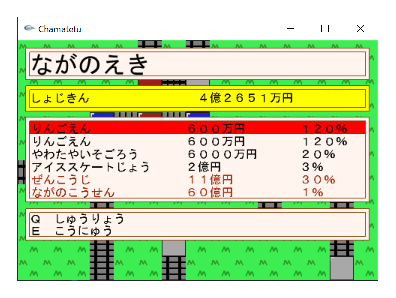
\includegraphics[scale=1.5]{bukkenex.eps}
        \caption{物件の例(長野駅)}
         \label{bukkenex}
        \end{figure}
    
    \subsection{ゲームの進行方法}
    ゲームの進行について説明する.ここではゲームの進行の概要について説明し,実際の画面表示については実装部分と共に述べる.
    図\ref{processgame}にゲーム進行のフローチャートを示す.ゲームを開始すると,初期設定が行われ,タイトル画面が表示される.
    初期設定としてはゲームスタート時の駅の設定および年月の設定が行われる.ゲームスタート時の駅は長野駅,年月は「1年目4月」に設定が行われる仕様にした.
    次に目的地の設定が行われる.目的地の処理の詳細については!で述べる.目的地の設定が完了するとゲームのメイン部分である社長の行動が始まる.各社長はターン中に
    サイコロを1つふって出た目の数だけ進む,もしくはカードを使う,のどちらかの行動を行うことができる.各社長が1回行動すると,年月の経過処理として1ヵ月経過する処理が行われる.
    年月の経過処理後の処理は月によって変化する.3月でない場合は再び社長の行動の処理が行われる.3月の場合は社長の行動の前に「決算」という処理が行われる.決算の処理については!で述べる.
    さらに3年目の場合は決算として最終成績が表示されゲームの終了処理が行われる.
    \begin{figure}[H]
        \centering
        
\includegraphics[scale=2.3]{processgame.eps}
        \caption{ゲームの進行}
         \label{processgame}
        \end{figure}

    \subsection{マップの設定}
    マップの設定について説明する.図\ref{map}に本ゲームのマップを示す.図\ref{map}の地名からも読み取れるように,本ゲームは長野県を舞台にしている.
    ただし,実際のゲームでは駅名は表示されない仕様になっている.マップは32$\times$32の画像を敷き詰める形で描画しており,サイズは960$\times$960である.
    なお,ウィンドウサイズは幅480,高さ320のため実際のゲームでは,行動中の社長を中心として画面におさまる部分だけを描画している.

    \begin{figure}[H]
        \centering
        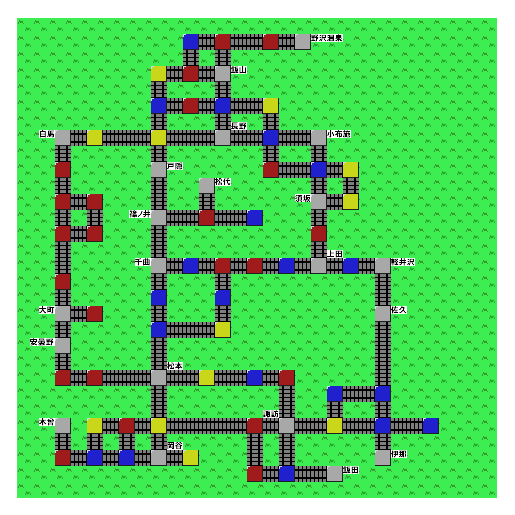
\includegraphics[scale=1.9]{map.eps}
        \caption{ゲームのマップ}
         \label{map}
        \end{figure}

    マップを描画する画像には表\ref{mapimage}に示す種類のものがある.
    これらの画像は「/mapparts」に保存されている.背景は季節によって変化する.月と季節は次に示すようになっている.図\ref{map}の
    マップは背景が春の場合である.季節ごとに背景が変化する仕様は桃鉄を参考にした.
    \begin{itemize}
        \item 春 : 3月~5月 
        \item 夏 : 6月~8月 
        \item 秋 : 9月~11月 
        \item 冬 : 12月~2月 
      \end{itemize}

\begin{table}[H]
  \caption{マップとして描画される画像の種類}
\label{mapimage}
\begin{center}
    \begin{tabular}{c|c|c}\hline
        画像の意味 & 画像のファイル名 & 実際の色や模様 \\ \hline \hline
        背景(春) & season1.png & 明るい緑 \\ 
        背景(夏) & season2.png & 濃い緑 \\
        背景(秋) & season3.png & 茶色 \\
        背景(冬) & season4.png & 白 \\
        プラス駅 & map1.png & 青 \\
        マイナス駅 & map2.png & 赤 \\
        カード駅 & map3.png & 黄色 \\
        物件駅 & map4.png & 灰色 \\ 
        線路(縦) & map5.png & 灰色背景に黒の線路 \\ 
        線路(横) & map6.png & 灰色背景に黒の線路 \\ 
        目的地駅 & map7.png & 灰色背景に駅のマーク\\ \hline
    \end{tabular}
\end{center}
\end{table}

    \subsection{駅の設定}
    駅の設定について説明する.サイコロをふって移動した社長が停車できる駅の種類には,表\ref{mapimage}に示したように,「プラス駅」,「マイナス駅」,「カード駅」,「物件駅」,「目的地駅」の5つがある.
    プラス駅は停車するとお金がもらえる駅である.もらえるお金は夏が最も多く,冬が最も少ない仕様になっている.マイナス駅は停車すると所持金が減少する駅である.
    減少する金額は夏が最も少なく,冬が最も多い仕様になっている.減少する額によっては所持金が負になる,いわゆる借金という状態になることがある.この場合,
    物件を売却することで借金を返済する処理が行われる.本ゲームでの借金の返済は売却する物件を選択する方式ではなく,自動で売却する物件を選ぶ方式を採用した.
    売却する物件の優先順位は次に示す通りである.なお,所持している全ての物件を売却しても借金が返済できない場合は所持金が負となった状態でターンが終了する.
    \begin{enumerate}
        \item 独占している駅の物件でなく,借金額よりも価格が高い物件
        \item 独占している駅の物件でなく,借金額よりも価格が低い物件
        \item 独占している物件で,借金額よりも価格が高い物件
        \item 独占している物件で,借金額よりも価格が低い物件
    \end{enumerate}
     カード駅は停車するとカードがもらえる駅である.カードは5枚まで所持することができ,カード駅に停車したときに既に5枚カードを持っている場合,この処理はスキップされる.
    カードは表\ref{cardlist}に示す8種類がある.カード名は桃鉄を参考にした.表\ref{cardlist}のカードのうち,急行カード,特急カード,新幹線カードの3種類は
    カードを仕様したあとにサイコロをふって移動することができる.他のカードについは,成功,失敗にかかわらずターンが終了する.
    \begin{table}[H]
        \caption{カード名と効果}
      \label{cardlist}
      \begin{center}
          \begin{tabular}{c|c}\hline
              カード名 & カードの効果 \\ \hline \hline
              急行カード & サイコロが2個に増える.\\
              特急カード & サイコロが3個に増える.\\
              新幹線カード & サイコロが4個に増える.\\
              サミットカード & すべての社長を自分のマスに集める.3分の2の確率で成功する.\\
              ぶっとびカード & ランダムな物件駅に移動する. \\
              10億円カード & 10億円が手に入る.\\
              徳政令カード & 借金を負っている社長の所持金が0円になる.\\
              剛速球カード & 他の社長のカードをすべて破棄する.2分の1の確率で成功する.\\ \hline
          \end{tabular}
      \end{center}
      \end{table}

      \subsection{決算の処理}
      決算の処理について説明する.決算は3月が終了すると行われる処理である.決算は,所持している物件に応じて各社長の所持金が
      増加する処理である.ある社長が決算で得られる金額$S$を計算する方法について説明する.物件を$n$個持っており,所持している$i$番目の物件の価格$p_i$,
      収益率$r_i$,その物件が所属する駅が自分の独占のとき$d_i=2$,独占でないとき$d_i=1$とする.このとき,決算で得られる金額$S$は式(\ref{kessan})で表せる.
      \begin{equation}
        S = \sum_{i=1}^{n} \frac{p_i r_i d_i}{100}
        \label{kessan}
      \end{equation}
      例えば,ある社長が,図\ref{bukkenex}の「やわたやいそごろう」と「アイススケートじょう」を所持している場合に
      決算でもらえる金額を計算してみる.式(\ref{kessan})に値を代入して計算を行うと,式(\ref{kessan_ex1})に示すように1800万円になる.
      この例では独占はしていないから$d_i$は常に1である.

      \begin{eqnarray}
        S &=& \sum_{i=1}^{n} \frac{p_i r_i d_i}{100} \\
          &=& \frac{1}{100} \left( 6000\times10^4 \cdot 20 + 20000\times10^4 \cdot 3 \right) \\
          &=& 1800 \times10^4
        \label{kessan_ex1}
      \end{eqnarray}    
       本ゲームは3年決戦であるため,3年目の決算は「最終成績」という形で表示される.最終成績を表示した後はゲームを終了するように促す画面を表示する.
    
      \section{実行環境とビルド方法}
      本章では,実行環境,ビルド方法,ディレクトリ構造の3つについて述べる.
      \subsection{実行環境}
      実行環境を\ref{env}に示す.gccとは「GNU Compiler Collection」の略称で,GNUプロジェクトが公開しているコンパイラのことである.
      makeはMakefileにプログラムのコンパイルやリンクの方法を指示することで,コンパイルを簡単に行うことができるツールのことである.
      makeを用いることは,gccコンパイル時に,長いオプションを入力しなくてよい,ファイルの更新を取得して必要なものだけをコンパイルしてくれる
      という利点がある.
      
      \begin{table}[H]
        \caption{実行環境}
      \label{env}
      \begin{center}
          \begin{tabular}{c|l}\hline
            CPU & Intel(R) Core(TM) i7-6500U 2.50GHz  \\ 
            メモリ & 16.0GB DDR4 \\
            OS & Microsoft Windows 10 Home \\
            gcc &  version 9.3.0 \\
            make & version 4.3 \\ \hline
          \end{tabular}
      \end{center}
      \end{table}
      
      \subsection{ビルド方法}
      ビルド方法について説明する.まず,「j17406.tar.gz」を保存したディレクトリに移動する.次にリスト\ref{kaito}に示すコマンドを実行する.
      リスト\ref{kaito}のコマンドを実行することで,j17406.tar.gzが解凍される.
      \begin{lstlisting}[basicstyle=\ttfamily\footnotesize, frame=single,label=kaito,caption=j17406.tar.gzの解凍]
gzip -dv j17406.tar.gz
tar xvf j17406.tar
        \end{lstlisting}
        解凍を行えたから,リスト\ref{make}の1行目のコマンドを実行してビルドを行う.リスト\ref{make}のコマンドを実行して
        「j17406.exe」が生成されていればビルド成功である.「j17406.exe」の実行はリスト\ref{make}の2行目のコマンドで行う.
        リスト\ref{make}の2行目のコマンドを実行して図\ref{sp4}に示す画面が表示されれば,ゲームの起動が成功している.
        \begin{lstlisting}[basicstyle=\ttfamily\footnotesize, frame=single,label=make,caption=makeコマンド]
make
.\j17406.exe
        \end{lstlisting}  

    \begin{figure}[H]
        \centering
        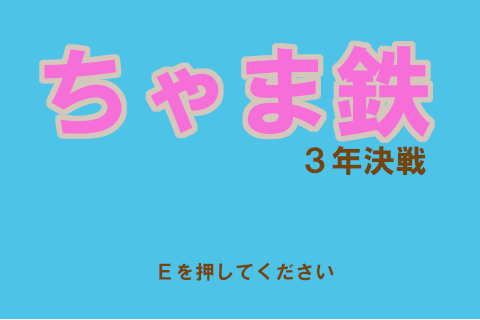
\includegraphics[scale=1.8]{sp4.png}
        \caption{ゲームのスタート画面}
         \label{sp4}
        \end{figure}

      \subsection{ディレクトリ構造}
      リスト\ref{tree}に「/j17406」のディレクトリ構造を示す.リスト\ref{tree}はtreeコマンドを用いてディレクトリ構造を
      表示したものである.ここでは,深さ1のファイル,ディレクトリのみを表示している.なぜなら,日本語画像や物件情報を保存しているディレクトリがあるため全てのファイルを
      表示すると見にくくなってしまうからである.
      ゲームの実装のためのコードは「game.c」および「j17406.c」に記述している.また,関数,定数の定義は
      「game.h」に記述している.画像は,画像の種類ごとにディレクトリを分けて保存している.ディレクトリ名と保存している画像の種類は
      表\ref{imgdir}の通りである.property.txtおよび「/property」に保存されているtxtファイルは駅の情報および物件の情報を保存している.
    
        \begin{lstlisting}[basicstyle=\ttfamily\footnotesize, frame=single,label=tree,caption=ディレクトリ構造]
j17406
├── Makefile
├── charimg
├── description.html
├── descriptionimg
├── dice
├── eventparts
├── game.c
├── game.h
├── icon.o
├── j17406.c
├── mapparts
├── property
├── property.txt
└── readme.txt
        \end{lstlisting}    
        
      \begin{table}[H]
        \caption{画像を保存するディレクトリ}
      \label{imgdir}
      \begin{center}
          \begin{tabular}{c|c}\hline
            ディレクトリ名 & 保存している画像の種類 \\ \hline \hline
            charimg & 日本語を画面に表示するための画像 \\
            dice & サイコロの画像 \\ 
            eventparts & 社長の画像,スタート画面,決算,ゲーム終了画面 \\ 
            mapparts & マップ描画のための画像 \\
            descriptionimg & description.htmlのための画像 \\ \hline
          \end{tabular}
      \end{center}
      \end{table}
        
    
    \section{プログラムの説明と実行結果}
    本章では次に示すプログラムの説明および実行結果について述べる.なお,プログラム中に登場する定数の値は付録の
    「game.h」(リスト!)を参照してほしい.
    \begin{enumerate}
        \item playerstatus構造体
        \item propertystatus構造体
        \item stationstatus構造体
        \item Map配列の定義
        \item 日本語プロトコルの定義
        \item 画像の読み込み
        \item 画像および日本語の表示
        \item 駅および物件情報の読み込み
        \item メイン関数(j17406.c)
        \item ウィンドウサイズ変更への対応(Reshape関数)
        \item ゲームの進行状況管理
        \item キーボード入力の処理
        \item ゲームの初期化とタイトル画面の表示
        \item 目的地の設定処理
        \item プレイヤーおよびマップの描画処理
        \item ターンのはじめの処理
        \item サイコロをふる処理
        \item マス移動および停車駅の判定処理
        \item 物件駅の処理
        \item プラス駅の処理
        \item マイナス駅および借金の処理
        \item カード駅の処理
        \item ターン終了時の処理
        \item 決算および最終成績の処理
    \end{enumerate}    

    \subsection{playerstatus構造体}
    playerstatus構造体の定義と初期化について説明する.まず,playerstatus構造体の定義について説明する.
    playerstatus構造体は一人の社長の情報を保持するための構造体である.リスト\ref{playerstatus}に「game.h」におけるplayerstatus構造体の
    定義を示す. playerstatus構造体は「社長名」,「所持金」,「総資産」,「現在の座標(x,y)」,「カード枚数」,「カードの通し番号」の7つをメンバとして持っている.
    所持金および総資産は万円単位で扱うものとする.例えば所持金が「2200万円」場合,メンバmoneyには2200が代入される.これ以降にも金額を
    扱うための変数が登場するが,そのすべての変数は万円単位で扱うものとする.
    また,11行目のようにplayerstatus構造体の配列を定義することで,プレイ人数3人分の情報を保持する構造体の配列を作成している.
    \begin{lstlisting}[basicstyle=\ttfamily\footnotesize, frame=single,label=playerstatus,caption=playerstatus構造体の定義と初期化]
// プレイヤーの情報構造体
struct playerstatus{
    char name[NAMEMAX]; // プレイヤー名
    int money; // 所持金
    int assets; // 総資産
    int x; // x座標(実描画座標)
    int y; // y座標(実描画座標)
    int cardnum; // 持っているカード枚数
    int card[CARDMAX]; // カードの番号記憶
};
    
    typedef struct playerstatus player;
    player players[PLAYERNUM]; // 人数分の配列を確保
    \end{lstlisting}

    次にplayerstatus構造体を初期化する関数について説明する.リスト\ref{InitPlayer}に,playerstatus構造体を初期化する関数である
    InitPlayer関数のコードを示す.InitPlayer関数の内部では,for文を用いてplayerstatus構造体の配列を初期化している.
    リスト\ref{InitPlayer}中の定数の値はINITXが416(13$\times$32),INITYが224(7$\times$32),INITMONEYは10000である.
    座標(13,7)はMap配列における長野駅の座標である.playerstatus構造体の座標(x,y)は画面に描画する実座標を
    保持する仕様にしているため画像サイズである32倍している.
    \begin{lstlisting}[basicstyle=\ttfamily\footnotesize, frame=single,label=InitPlayer,caption=InitPlayer関数]
// プレイヤー構造体を初期化
void InitPlayer(void){
    int i,j;
    for(i=0;i<PLAYERNUM;i++){
        //プレイヤーhoge
        sprintf(players[i].name,"llpureiiyallms%d",i+1);
        players[i].x=INITX;
        players[i].y=INITY;
        players[i].money=INITMONEY;
        players[i].assets=0;
        players[i].cardnum=0;
        for(j=0;j<CARDMAX;j++){
            players[i].card[j]=0;
        }
    }
}
            \end{lstlisting}

    \subsection{propertystatus構造体}
    propertystatus構造体は一つの物件の情報を保持するための構造体である.「game.h」におけるpropertystatus構造体の定義をリスト\ref{propertystatus}に示す.
    propertystatus構造体は「物件名」,「物件保持者」,「価格」,「収益率」の4つをメンバとして持っている.物件保持者は表\ref{whohold}のルールで扱うものとする.
   \begin{lstlisting}[basicstyle=\ttfamily\footnotesize, frame=single,label=propertystatus,caption=propertystatus構造体の定義]
   // 物件情報構造体
   struct propertystatus{
   char name[STRMAX]; // 物件名
   int holder; // 物件所持者
   int price; // 価格
   int earnings; // 収益率
   };
   
   typedef struct propertystatus property;
   \end{lstlisting}
   
   \begin{table}[H]
     \caption{物件保持者メンバの意味}
   \label{whohold}
   \begin{center}
       \begin{tabular}{c|c}\hline
       値 & 保持者 \\ \hline \hline
         0 & 保持者なし \\
         1 & 社長1 \\
         2 & 社長2 \\
         3 & 社長3 \\ \hline
       \end{tabular}
   \end{center}
   \end{table}

    \subsection{stationstatus構造体}
stationstatus構造体は一つの駅の情報を保持するための構造体である.リスト\ref{stationstatus}にstationstatus構造体の定義を示す.
stationstatus構造体は,「駅名」,「駅の座標(x,y)」,「独占フラグ」,「物件の数」,「propertystatus構造体の配列」の6つをメンバとして持つ.
駅の座標(x,y)はplayerstatus構造体のような実座標ではなく,マップを描画するための配列のインデックスである.独占フラグは
その駅を誰が独占しているかを判別するために用いる.独占フラグの値とその意味は表\ref{whohold}と同じである.
\begin{lstlisting}[basicstyle=\ttfamily\footnotesize, frame=single,label=stationstatus,caption=stationstatus構造体の定義と初期化]
// 駅情報構造体
struct stationstatus{
char name[STRMAX]; // 駅名
int x; // x座標
int y; // y座標
int ismonopoly; // 独占フラグ
int propertynum; // 物件数
property plist[PROPERTMAX]; // 物件情報構造体の配列
};

typedef struct stationstatus station;
station stations[STATIONNUM]; // 駅の数分の配列を確保
station distination; // 目的地配列
\end{lstlisting}

    \subsection{Map配列の定義}
    マップの情報はMap配列が保持している.Map配列の定義をリスト\ref{Maparray}に示す.
    マップのサイズは30$\times$30で,配列のサイズは30$\times$31である.
    x方向の配列のサイズが1大きいのは,null文字を格納するためである.Map配列の文字列は
    「A」,「B」,「C」,「P」,「M」,「-」,「\textbar」のいずれかの文字から構成されている.表\ref{mapstr}に
    文字と実際に表示される画像の関係を示す.
    \begin{lstlisting}[basicstyle=\ttfamily\footnotesize, frame=single,label=Maparray,caption=Map配列の定義]
// マップ配列
char Map[YMAX][XMAX+1] = { //NULL文字に気を付ける
       //012345678901234567890123456789      
        "AAAAAAAAAAAAAAAAAAAAAAAAAAAAAA", // 0
        "AAAAAAAAAAAP-M--M-BAAAAAAAAAAA", // 1
        "AAAAAAAAAAA|A|AAAAAAAAAAAAAAAA", // 2
        "AAAAAAAAAC-M-BAAAAAAAAAAAAAAAA", // 3
        "AAAAAAAAA|AAA|AAAAAAAAAAAAAAAA", // 4
        "AAAAAAAAAP-M-P--CAAAAAAAAAAAAA", // 5
        "AAAAAAAAA|AAA|AA|AAAAAAAAAAAAA", // 6
        "AAAB-C---C---B--P--BAAAAAAAAAA", // 7
        "AAA|AAAAA|AAAAAA|AA|AAAAAAAAAA", // 8
        "AAAMAAAAABAAAAAAM--P-CAAAAAAAA", // 9
        "AAA|AAAAA|AABAAAAAA|A|AAAAAAAA", // 0
        "AAAM-MAAA|AA|AAAAAAB-CAAAAAAAA", // 1
        "AAA|A|AAAB--M--PAAA|AAAAAAAAAA", // 2
        "AAAM-MAAA|AAAAAAAAAMAAAAAAAAAA", // 3
        "AAA|AAAAA|AAAAAAAAA|AAAAAAAAAA", // 4
        "AAA|AAAAAB-P-M-M-P-B-P-BAAAAAA", // 5
        "AAAMAAAAA|AAA|AAAAAAAAA|AAAAAA", // 6
        "AAA|AAAAAPAAAPAAAAAAAAA|AAAAAA", // 7
        "AAAB-MAAA|AAA|AAAAAAAAABAAAAAA", // 8
        "AAA|AAAAAP---CAAAAAAAAA|AAAAAA", // 9
        "AAABAAAAA|AAAAAAAAAAAAA|AAAAAA", // 0
        "AAA|AAAAA|AAAAAAAAAAAAA|AAAAAA", // 1
        "AAAM-M---B--C--P-MAAAAA|AAAAAA", // 2
        "AAAAAAAAA|AAAAAAA|AAP--PAAAAAA", // 3
        "AAAAAAAAA|AAAAAAA|AA|AA|AAAAAA", // 4
        "AAABAC-M-C-----M-B--C--P--PAAA", // 5
        "AAA|A|A|A|AAAAA|A|AAAAA|AAAAAA", // 6
        "AAAM-P-P-B-CAAA|A|AAAAABAAAAAA", // 7
        "AAAAAAAAAAAAAAAM-P--BAAAAAAAAA", // 8
        "AAAAAAAAAAAAAAAAAAAAAAAAAAAAAA"  // 9
};
    \end{lstlisting}

    \begin{table}[H]
        \caption{文字と画像の対応}
      \label{mapstr}
      \begin{center}
          \begin{tabular}{c|c}\hline
            文字 & 表示される画像 \\ \hline \hline
            A & 背景 \\ 
            B & 物件駅 \\ 
            C & カード駅 \\ 
            P & プラス駅 \\ 
            M & マイナス駅 \\ 
            - & 線路(横) \\ 
            \textbar  & 線路(縦) \\ \hline
          \end{tabular}
      \end{center}
      \end{table}

    \subsection{日本語プロトコルの定義}
    桃鉄をイメージしたゲームを実装するうえで,日本語を画面に表示できなければ,ローマ字が並んでわかりにくい.しかしGLUTは日本語に対応していない.
そこで画像を用いて日本語をゲーム画面に描画する機能を作成した.これを日本語プロトコルと呼ぶことにする.文字色は黒と赤のどちらかで描画することが可能である.
作成した日本語プロトコルでは次に示す文字を画面に表示することができる.一部のアルファベット,記号,漢字をまとめて特殊文字と呼ぶことにする.
\begin{itemize}
  \item 50音(ひらがな,カタカナ)
  \item 濁音(ひらがな,カタカナ)
  \item 半濁音(ひらがな,カタカナ)
  \item 小文字(っ,ゃ,ゅ,ょ)(ひらがな,カタカナ)
  \item 数字
  \item 一部のアルファベット(W,A,S,D,E,Q)
  \item 一部の記号(読点,句点,\%,マイナスの記号(-),プラスの記号(+))
  \item ゲームに頻出する漢字(億,万,円)
\end{itemize}

これらの画像は「/charimg」に保存されている.画像のサイズはすべて32$\times$32pxである.画像名の意味は図\ref{howname}の通りである.
どの文字か判別する2文字はコード中で日本語を表示するための文字列に対応している.実際の文字と日本語プロトコルにおける文字の表現
方法は表\ref{jpp}の通りである.改行およびスペースは画像にはないが,画像を表示する位置を調整することで表現できる.表\ref{jpp}の情報は
game.cでリスト\ref{jpProtcolarray}に示すように定義されている.

\begin{figure}[H]
  \centering
  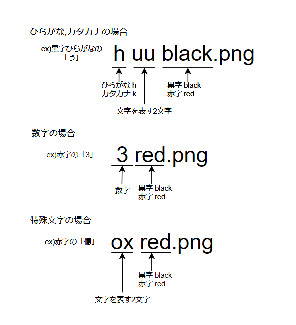
\includegraphics[scale=1.7]{howname.eps}
  \caption{画像の名前の意味}
   \label{howname}
  \end{figure}    

  \begin{table}[H]
    \caption{日本語プロトコルの文字表現}
  \label{jpp}
  \begin{center}
      \begin{tabular}{c|c|c|c|c}\hline
あ aa & い ii & う uu & え ee & お oo \\ 
か ka & き ki & く ku & け ke & こ ko \\ 
さ sa & し si & す su & せ se & そ so \\ 
た ta & ち ti & つ tu & て te & と to \\ 
な na & に ni & ぬ nu & ね ne & の no \\ 
は ha & ひ hi & ふ hu & へ he & ほ ho \\ 
ま ma & み mi & む mu & め me & も mo \\ 
や ya & -  & ゆ yu & -  & よ yo \\ 
ら ra & り ri & る ru & れ re & ろ ro \\ 
わ wa & -  & を wo & -  & ん nn \\ 
ゃ la & - & ゅ lu & っ lt & ょ lo \\ 
が ga & ぎ gi & ぐ gu & げ ge & ご go \\ 
ざ za & じ zi & ず zu & ぜ ze & ぞ zo \\
だ da & ぢ di & づ du & で de & ど do \\
ば ba & び bi & ぶ bu & べ be & ぼ bo \\ 
ぱ pa & ぴ pi & ぷpu &  ぺ pe & ぽ po \\ 
0  0 & 1  1 & 2  2 & 3  3 & 4  4 \\ 
5  5 & 6  6 & 7  7 & 8  8 & 9  9 \\ 
円 ex & 万 mx & 億 ox & \% px & - ms \\ 
+ ps & 句点 mr & 読点 tn & Q xq & W xw \\ 
E xe & A xa & S xs & D xd & - \\ 
改行 xx & スペース ss & - & - & - \\ \hline
      \end{tabular}
  \end{center}
  \end{table}
  
  \begin{lstlisting}[basicstyle=\ttfamily\footnotesize, frame=single,label=jpProtcolarray,caption=jpProtcol配列]
// 日本語プロトコル
char jpProtcol[JPMAX+SPMAX][3] = {"aa","ii","uu","ee","oo",
                        "ka","ki","ku","ke","ko",
                        "sa","si","su","se","so",
                        "ta","ti","tu","te","to",
                        "na","ni","nu","ne","no",
                        "ha","hi","hu","he","ho",
                        "ma","mi","mu","me","mo",
                        "ya","yu","yo",
                        "ra","ri","ru","re","ro",
                        "wa","wo","nn",
                        "lt","la","lu","lo",
                        "ga","gi","gu","ge","go",
                        "za","zi","zu","ze","zo",
                        "da","di","du","de","do",
                        "ba","bi","bu","be","bo",
                        "pa","pi","pu","pe","po",
                        "0","1","2","3","4","5"
                        ,"6","7","8","9",
                        "ex","mx","ox","px","ms","ps",
                        "mr","tn","xq","xw","xe","xa","xs","xd"
                        };

  \end{lstlisting} 
  
  \subsection{画像の読み込み}
  画像を読み込む方法について説明する.リスト\ref{readImg}に画像を読み込むためのreadImg関数のコードを示す.
  処理の内容はファイル名や読み込み先を変えて画像を読み込んでいるだけだから,リスト\ref{readImg}の7行目から11行目のイベントマップの読み込みを
  例に説明する.画像を読み込むためには2つの変数が必要である.今の例ではspimgとspinfoである.変数spimgには読み込んだ画像を識別するための値が
  代入され,変数spinfoには読み込んだ画像のと横幅,縦幅を代表とする情報が格納される.これらの変数にpngBind関数を用いて読み込んだ画像の
  情報を与えることで画像の読み込みを行っている.
  \begin{lstlisting}[basicstyle=\ttfamily\footnotesize, frame=single,label=readImg,caption=readImg関数]
// 画像読み込み
void readImg(void){
    int i;
    char fname[100];

    // イベントマップ読み込み
    for(i=0;i<SP_NUM;i++){
        sprintf(fname,".\\eventparts\\sp%d.png",i+1);
        spimg[i] = pngBind(fname, PNG_NOMIPMAP, PNG_ALPHA, 
       &spinfo[i], GL_CLAMP, GL_NEAREST, GL_NEAREST);        
    }

   // 季節マップ読み込み 
    for(i=0;i<SEASON_NUM;i++){
        sprintf(fname,".\\mapparts\\season%d.png",i+1);
        seasonimg[i] = pngBind(fname, PNG_NOMIPMAP, PNG_ALPHA, 
       &seasoninfo[i], GL_CLAMP, GL_NEAREST, GL_NEAREST);        
    }

    // マップイメージ読み込み
    for(i=0;i<=MAP_NUM;i++){
        sprintf(fname,".\\mapparts\\map%d.png",i+1);
        mapimg[i] = pngBind(fname, PNG_NOMIPMAP, PNG_ALPHA, 
       &mapinfo[i], GL_CLAMP, GL_NEAREST, GL_NEAREST);
    }
    // プレイヤー画像を読み込み
    for(i=0;i<PLAYERNUM;i++){
        sprintf(fname,".\\eventparts\\player%d.png",i+1);
        playerimg[i] = pngBind(fname, PNG_NOMIPMAP, PNG_ALPHA, 
       &playerinfo[i], GL_CLAMP, GL_NEAREST, GL_NEAREST);
    }

    // サイコロの画像を読み込み
    for(i=0;i<DICEMAX;i++){
        sprintf(fname,".\\dice\\dice%d.png",i+1);
        diceimg[i] = pngBind(fname, PNG_NOMIPMAP, PNG_ALPHA, 
       &diceinfo[i], GL_CLAMP, GL_NEAREST, GL_NEAREST);
    }
    // read Hiragana black
    for(i=0;i<JPMAX;i++){
        sprintf(fname,".\\charimg\\h%sblack.png",jpProtcol[i]);
        hblackimg[i] = pngBind(fname, PNG_NOMIPMAP, PNG_ALPHA, 
        &hblackinfo[i], GL_CLAMP, GL_NEAREST, GL_NEAREST);
    }

    // read Hiragana red
    for(i=0;i<JPMAX;i++){
        sprintf(fname,".\\charimg\\h%sred.png",jpProtcol[i]);
        hredimg[i] = pngBind(fname, PNG_NOMIPMAP, PNG_ALPHA, 
        &hredinfo[i], GL_CLAMP, GL_NEAREST, GL_NEAREST);
    }
    // read Katakana black
    for(i=0;i<JPMAX;i++){
        sprintf(fname,".\\charimg\\k%sblack.png",jpProtcol[i]);
        kblackimg[i] = pngBind(fname, PNG_NOMIPMAP, PNG_ALPHA, 
        &kblackinfo[i], GL_CLAMP, GL_NEAREST, GL_NEAREST);
    }
    // read Katakana red
    for(i=0;i<JPMAX;i++){
        sprintf(fname,".\\charimg\\k%sred.png",jpProtcol[i]);
        kredimg[i] = pngBind(fname, PNG_NOMIPMAP, PNG_ALPHA, 
        &kredinfo[i], GL_CLAMP, GL_NEAREST, GL_NEAREST);
    }
    // read Special Str red
    for(i=JPMAX;i<JPMAX+SPMAX;i++){
        sprintf(fname,".\\charimg\\%sred.png",jpProtcol[i]);
        hredimg[i] = pngBind(fname, PNG_NOMIPMAP, PNG_ALPHA, 
        &hredinfo[i], GL_CLAMP, GL_NEAREST, GL_NEAREST);
    }
    // read Special Str black
    for(i=JPMAX;i<JPMAX+SPMAX;i++){
        sprintf(fname,".\\charimg\\%sblack.png",jpProtcol[i]);
        hblackimg[i] = pngBind(fname, PNG_NOMIPMAP, PNG_ALPHA, 
        &hblackinfo[i], GL_CLAMP, GL_NEAREST, GL_NEAREST);
    }
}
      \end{lstlisting} 
  \subsection{画像および日本語の表示}  
  画像および日本語をゲーム画面に表示する方法について説明する.まず,画像を表示する方法について説明する.画像の表示
  はリスト\ref{PutSprite}に示すPutSprite関数を用いて行っている.PutSprite関数は「Springs of C」!から引用した関数である.
  リスト\ref{PutSprite}のコードでは,引用した関数に,引数として画像の表示倍率scaleを加え,画像の縮小を行えるようにした.
  画像の表示倍率はリスト\ref{PutSprite}の6行目および7行目でテクスチャの幅と高さをscale倍することで行っている.
  \begin{lstlisting}[basicstyle=\ttfamily\footnotesize, frame=single,label=PutSprite,caption=PutSprite関数]
// (x,y)に大きさscaleの画像を表示
void PutSprite(int num, int x, int y, pngInfo *info,double scale)
{
    int w, h;  //  テクスチャの幅と高さ

    w = info->Width*scale;   //  テクスチャの幅と高さを取得する
    h = info->Height*scale;

    glPushMatrix();
    glEnable(GL_TEXTURE_2D);
    glBindTexture(GL_TEXTURE_2D, num);
    glColor4ub(255, 255, 255, 255);

    glBegin(GL_QUADS);  //  幅w, 高さhの四角形

    glTexCoord2i(0, 0); 
    glVertex2i(x, y);

    glTexCoord2i(0, 1);
    glVertex2i(x, y + h);

    glTexCoord2i(1, 1);
    glVertex2i(x + w, y + h);

    glTexCoord2i(1, 0);
    glVertex2i(x + w, y);

    glEnd();

    glDisable(GL_TEXTURE_2D);
    glPopMatrix();
}
          \end{lstlisting} 

    次に日本語の表示方法について説明する.リスト\ref{jpfunc}に日本語を表示するための関数であるdrawChar関数および
    drawString関数のコードを示す.drawChar関数は「1文字」の日本語を表示する関数であり,drawString関数はdrawChar関数を
    連続して呼び出して文字列を表示する関数である.drawChar関数は引数としてjpProtcol配列(リスト\ref{jpProtcolarray})の
    インデックスnum,ひらがな/カタカナのどちらで表示するかを示すkh,黒/赤のどちらで描画するかを示すcolor,描画する実座標(x,y),
    表示倍率scaleの6つを受け取る.引数khは0のときひらがな,1のときカタカナである.引数colorは0のとき黒,1のとき赤である.
    drawChar関数の内部では,受け取った引数から表示する文字の種類を判断し,PutSprite関数で描画する処理を行っている.\\
     drawString関数は引数として描画する文字列string,文字色color,実座標(x,y),表示倍率scaleの5つを受け取る.drawString関数
    の内部では,まず引数として受け取った文字列stringを1文字または2文字ずつ取り出して,文字の種類を判断している.リスト\ref{jpfunc}では,
    29行目および30行目が数字かどうかの判別を行っている部分である.日本語の判別は35行目,特殊文字は41行目で判定している.例外として
    ひらがな/カタカナ切り替えは47行目,改行は51行目で判定している.空白は判定していないが,これは該当する文字がない場合に何も
    描画せずに文字を表示する位置がずれることを利用している.このため,空白は「ss」以外の文字列でも表現できるがコードのわかり
    やすさという観点から「ss」という文字に統一している.文字の種類の判断が行えたら,jpProtcol配列におけるその文字のインデックス
    および描画のための情報をdrawChar関数に渡して描画を行っている.最後に58行目から63行目で次に表示する文字の位置を計算する処理
    を行っている.これらの処理によって画面に日本語を描画している.

    \begin{lstlisting}[basicstyle=\ttfamily\footnotesize, frame=single,label=jpfunc,caption=日本語表示のための関数]
// 1文字の日本語を表示
// int kh : 0,Hiragana 1,Katakana
// int color 0,black 1,red
void drawChar(int num,int kh,int color,int x,int y,double scale){
    if(kh==0){
        if(color==0){ // hiragana black
            PutSprite(hblackimg[num], x, y, &hblackinfo[num],scale);
        }else{ //hiragana red
            PutSprite(hredimg[num], x, y, &hredinfo[num],scale);
            }
        }else{ 
        if(color==0){ // katakana black
            PutSprite(kblackimg[num], x, y, &kblackinfo[num],scale);
        }else{ // katakana red
            PutSprite(kredimg[num], x, y, &kredinfo[num],scale);
        }
    }
}

// 引数stringの文字列を表示
void drawString(char *string,int color,int xo,int yo,double scale){
    int i,j;
    int len = strlen(string);
    int x=xo;
    int y=yo;
    int flg;
    int kh=0;
    for(i=0;i<len;i++){
        flg=string[i]-'0'; // インデクス計算
        if((flg>=0)&&(flg<=9)){ // 数字描画
            drawChar(JPMAX+flg,0,color,x,y,scale);
            flg=1;
        }else{
            for(j=0;j<JPMAX;j++){ //日本語描画
                if((jpProtcol[j][0]==string[i])&&(jpProtcol[j][1]==string[i+1])){
                    drawChar(j,kh,color,x,y,scale);
                    break;
                }
            }       
            for(j=JPMAX+10;j<JPMAX+SPMAX;j++){ //特殊文字描画
                if((jpProtcol[j][0]==string[i])&&(jpProtcol[j][1]==string[i+1])){
                    drawChar(j,kh,color,x,y,scale);
                    break;
                }
            }
            flg=1;
            if((string[i]=='l')&&(string[i+1]=='l')){ //ひらがな/カタカナ切り替え
                kh=1-kh;
                flg=0;
            }
            if((string[i]=='x')&&(string[i+1]=='x')){ // 改行
                x=xo;
                flg=0;
                y+=IMGSIZE*scale;
            }     
            i++;
        }
        if(flg==1){ // 次の座標に移動
            x+=IMGSIZE*scale;
            if(x>InitWidth-22){
                x=xo;
                y+=IMGSIZE*scale;
            }
        }
    }
}

                  \end{lstlisting} 
  \subsection{駅および物件情報の読み込み}
  駅および物件の情報を読み込む方法について説明する.動作確認は次節のメイン関数で行う.まず,駅の情報を読み込む方法について説明する.
  駅の情報はproperty.txtに保存されている.リスト\ref{propertytxt}にproperty.txtの内容を示す. property.txt
  は「駅名 x座標,y座標」という形式ですべての駅の情報が保存されている.駅名は日本語プロトコルにおける
  駅名の表示である.座標は実座標ではなく, Map配列(リスト\ref{Maparray})のインデックスである.
  例えば飯山駅の場合,駅名が「iiiiyama」, Map配列における座標が(13,3)になっている.リスト\ref{Maparray}の(13,3)を確認すると
  「B」つまり物件駅になっている.また,図\ref{map}からこの位置にある駅は飯山駅であることがわかる.これらよりproperty.txtで
  定義した駅名および座標が,Map配列や画面表示と合致していることが確認できた.同様にして全ての駅について
  駅名と座標が間違っていないことを筆者は確認した.
\begin{lstlisting}[basicstyle=\ttfamily\footnotesize, frame=single,label=propertytxt,caption=property.txt]
nozawaoonnsenn 18,1
iiiiyama 13,3
togakusi 9,9
nagano 13,7
oobuse 19,7
suzaka 19,11
matusiro 12,10
sinonoii 9,12
hakuba 3,7
oooomati 3,18
tikuma 9,15
uueeda 19,15
karuiizawa 23,15
aadumino 3,20
saku 23,18
matumoto 9,22
suwa 17,25
kiso 3,25
ookaya 9,27
iiiida 20,28
iina 23,27
        \end{lstlisting}   
    
    property.txtの形式が確認できたから,これを読み込む関数について説明する.リスト\ref{readStation}に駅の情報を読み込むための関数
    であるreadStation関数のコードを示す.リスト\ref{readStation}においてファイルから読み取った情報をstationstatus構造体に代入しているのは
    11行目から14行目である.11行目でfscanf関数を用いて「駅名 x座標,y座標」という情報を構造体に代入している.
\begin{lstlisting}[basicstyle=\ttfamily\footnotesize, frame=single,label=readStation,caption=readStation関数]
// ファイルから駅情報を取得
// stations構造体を初期化
void readStation(void){
    FILE *fp;
    int i=0;
    fp=fopen("property.txt","r");
    if(fp==NULL){ // 開けなかったとき
        printf("file not found");
        exit(0);
    }else{ // 駅名と座標を取得
        while(fscanf(fp,"%s %d,%d",stations[i].name,&stations[i].x,&stations[i].y)!=EOF){
            stations[i].ismonopoly=0; // 独占フラグ初期化
            i++;
        }
        fclose(fp);
    }
}

        \end{lstlisting}     
    
    次に物件の情報を読み込む方法について説明する.物件の情報は「/property」に「駅名.txt」という形式で保存している.
    駅名は日本語プロトコルにおける駅名である.
    リスト\ref{naganotxt}およびリスト\ref{matumototxt}に物件情報を保存しているファイルの例を示す.リスト\ref{naganotxt}は
    長野駅,リスト\ref{matumototxt}は松本駅である.物件の情報は「物件名 価格,収益率」という形式で保存している.
\begin{lstlisting}[basicstyle=\ttfamily\footnotesize, frame=single,label=naganotxt,caption=/property/nagano.txt]
rinngoeenn 600,120
rinngoeenn 600,120
yawatayaiisogorouu 6000,20 
llaaiisusukellmslltollzilouu 20000,3 
zennkouuzi 110000,30
naganokouusenn 600000,1
\end{lstlisting}  

\begin{lstlisting}[basicstyle=\ttfamily\footnotesize, frame=single,label=matumototxt,caption=/property/matumoto.txt]
giluuuniluuullpannll 1200,130 
kamikouuti 12000,80
sinnsiluuudaiigaku 60000,30
aasamaoonnsenn 80000,4
kiluuukaiitigaltkouu 90000,5
matumotozilouu 150000,5
\end{lstlisting}     

    物件情報の保存形式が確認できたから,これを読み込む関数について説明する.リスト\ref{readProperty}に
    物件の情報を読み込む関数であるreadProperty関数のコードを示す.リスト\ref{readProperty}において
    ファイルから読み取った情報をpropertystatus構造体に代入しているのは,15行目および16行目である.
    readStation関数と同様にfscanf関数を用いて「物件名 価格,収益率」という情報を構造体に代入している.
    \begin{lstlisting}[basicstyle=\ttfamily\footnotesize, frame=single,label=readProperty,caption=readProperty関数]
// ファイルから物件情報を取得
void readProperty(void){
    FILE *fp;
    int i,j;
    char fname[100];
    for(i=0;i<STATIONNUM;i++){
        sprintf(fname,".\\property\\%s.txt",stations[i].name);
        fp=fopen(fname,"r");
        j=0;
        if(fp==NULL){ // 開けなかったとき
            printf("file not found in %s",stations[i].name);
            exit(0);
        }else{
            // 物件名,値段,収益率を取得
            while(fscanf(fp,"%s %d,%d",stations[i].plist[j].name,
            &stations[i].plist[j].price,&stations[i].plist[j].earnings)!=EOF){
            stations[i].plist[j].holder=0; // 購入フラグ初期化
            j++;
        }
        stations[i].propertynum=j; // 物件数を保存
        fclose(fp);
    }

    }   
}
                \end{lstlisting}     
  \subsection{メイン関数(j17406.c)}
メイン関数のコードについて説明する.リスト\ref{main}にメイン関数のコードを示す.
メイン関数ではウィンドウの生成,画像の読み込み,構造体の初期化を行う関数の実行,コールバック関数の登録,メインループ呼び出しの5つの処理を行っている.
ウィンドウの生成は12行目および13行目で行っている.12行目で生成するウィンドウのサイズを指定し,13行目で
ウィンドウを生成する処理を行っている.画像の読み込みの関数であるreadImg関数は23行目で実行している.
構造体の初期化は24行目から26行目で行っている.\\
 構造体の初期化が正確に行われていることを確認するために,
デバッグ用の関数としてdispPlayer関数およびdispStation関数を作成した.リスト\ref{debugfunc}にdispPlayer関数およびdispStation関数の
定義を示す.これらの関数はリスト\ref{main}の27行目および28行目で実行している.実際に提出したファイルではコメントアウトしているため
実行はされていない.dispPlayer関数は社長の情報を保持するplayerstatus構造体内容をすべてコンソール出力する関数である.
dispPlayer関数は引数として表示する範囲を指定できる変数detailがある.引数として0を与えるとすべての社長の情報を表示し,
1,2,3のいずれかを与えると表\ref{whohold}に対応する社長の情報のみが表示される.ここでは引数として0を与え,すべての
社長の情報を表示する機能のみを用いる.同様に,dispStation関数は駅および物件の情報を保持するstationstatus構造体およびpropertystatus構造体の内容を
すべて表示する関数である.dispStation関数も引数として表示する範囲を指定できる変数detailを持っている.引数として
0を与えた場合は全ての駅の情報を表示し,1以上の整数を与えた場合は,対応するインデックスの情報のみが表示される仕様になっている.
インデックスと駅の対応は,リスト\ref{propertytxt}の1行目の野沢温泉駅を0,2行目の飯山駅を1 $\cdots$というふうになっている.\\
リスト\ref{main}の32行目から35行目ではコールバック関数の登録を行っている.
コールバック関数とはキーボード入力や画面のリサイズを代表とするイベントが発生したときに実行される関数のことである. 
最後に37行目でglutMainLoop関数を実行することで,メインループを呼び出す処理を行っている.
    \begin{lstlisting}[basicstyle=\ttfamily\footnotesize, frame=single,label=main,caption=main関数]
#include <GL/glut.h>
#include <GL/glpng.h>
#include <stdio.h>
#include <stdlib.h>
#include <time.h>
#include "game.h"

int main(int argc, char **argv)
{
    srand((unsigned) time(NULL));
    glutInit(&argc, argv);
    glutInitWindowSize(InitWidth,InitHeight);
    glutCreateWindow("Chamatetu");
    glutInitDisplayMode(GLUT_RGBA | GLUT_ALPHA);
    glClearColor(1.0, 1.0, 1.0, 0.0);

    //  テクスチャのアルファチャネルを有効にする設定
    glEnable(GL_BLEND);
    glBlendFunc(GL_SRC_ALPHA, GL_ONE_MINUS_SRC_ALPHA);
    glTexEnvf(GL_TEXTURE_ENV, GL_TEXTURE_ENV_MODE, GL_MODULATE);
    
    // 画像読み込みと構造体の初期化
    readImg();
    InitPlayer();
    readStation();
    readProperty();
    dispPlayer(0); // デバッグ用
    dispStation(0); // デバッグ用
    turnstatus=0;
    inflg=0; // 進行状況を初期化
    //イベント登録
    glutReshapeFunc(Reshape);
    glutDisplayFunc(Display);
    glutKeyboardFunc(keyboard);
    glutTimerFunc(RESHAPETIME, Timer, 0);
    //  イベントループ突入
    glutMainLoop();

    return(0);
}
\end{lstlisting}  

    \begin{lstlisting}[basicstyle=\ttfamily\footnotesize, frame=single,label=debugfunc,caption=構造体の初期化を確認するための関数]
// デバッグ用関数 	
// プレイヤー構造体を表示	
// detail : 0 全部表示 , else その番号の駅を表示	
void dispPlayer(int detail){	
    int i,j;	
    if(detail==0){	
        for(i=0;i<PLAYERNUM;i++){	
            printf("--------------------\n");	
            printf("%s社長 (%d,%d)\n",players[i].name,
            players[i].x,players[i].y);	
            printf("\n");	
            printf("所持金 : %d\n",players[i].money);	
            printf("総資産 : %d\n",players[i].assets);
            printf("カード枚数 : %d\n",players[i].cardnum);
            for(j=0;j<CARDMAX;j++){
                printf("%d ",players[i].card[j]);
            }	
            printf("\n--------------------\n\n");	
        }	
    }else{	
        printf("--------------------\n");	
        printf("%s社長 (%d,%d)\n",players[detail-1].name,
        players[detail-1].x,players[detail-1].y);	
        printf("\n");	
        printf("所持金 : %d\n",players[detail-1].money);	
        printf("総資産 : %d\n",players[detail-1].assets);
        printf("カード枚数 : %d\n",players[detail-1].cardnum);
        for(j=0;j<CARDMAX;j++){
            printf("%d ",players[detail-1].card[j]);
        }		
        printf("\n--------------------\n\n");   	
    }	
}

// デバッグ用関数	
// 駅情報を表示	
void dispStation(int detail){	
    int i,j;	
    if(detail==0){	
        for(i=0;i<STATIONNUM;i++){	
            printf("--------------------\n");	
            printf("%s駅 (%d,%d)\n",stations[i].name,
            stations[i].x,stations[i].y);	
            printf("独占フラグ : %d   物件数 : %d\n",stations[i].ismonopoly,
            stations[i].propertynum);	
            for(j=0;j<stations[i].propertynum;j++){	
                printf("%s %d %d %d\n",stations[i].plist[j].name,
                stations[i].plist[j].price,stations[i].plist[j].earnings,
                stations[i].plist[j].holder);	
            }	
            printf("--------------------\n\n");	
        }	
        }else{	
        printf("--------------------\n");	
        printf("%s駅 (%d,%d)\n",stations[detail-1].name,stations[detail-1].x,
        stations[detail-1].y);	
        printf("独占フラグ : %d   物件数 : %d\n",stations[detail-1].ismonopoly,
        stations[detail-1].propertynum);	
        for(j=0;j<stations[detail-1].propertynum;j++){	
            printf("%s %d %d %d\n",stations[detail-1].plist[j].name,
            stations[detail-1].plist[j].price,stations[detail-1].plist[j].earnings,
            stations[detail-1].plist[j].holder);	
        }	
        printf("--------------------\n\n");     	
    }	
}
\end{lstlisting}

構造体の初期化が正確に行われていることを確認する.まず,playerstatus構造体について確認する.
初期化が正しく行えていれば,座標は(416,224),所持金は10000,それ以外のメンバには0が代入されているはずである.
リスト\ref{dispPlayerResult}にリスト\ref{main}を実行したときのコンソール画面を示す.
リスト\ref{dispPlayerResult}から全ての社長についてメンバに代入されている値が正しいことが確認できる.
これよりInitPlayer関数でplayerstatus構造体の初期化が正しく行えていることが確認できた.
\begin{lstlisting}[basicstyle=\ttfamily\footnotesize, frame=single,label=dispPlayerResult,caption=dispPlayer関数の実行結果]
--------------------
llpureiiyallms1社長 (416,224)

所持金 : 10000
総資産 : 0
カード枚数 : 0
0 0 0 0 0
--------------------

--------------------
llpureiiyallms2社長 (416,224)

所持金 : 10000
総資産 : 0
カード枚数 : 0
0 0 0 0 0
--------------------

--------------------
llpureiiyallms3社長 (416,224)

所持金 : 10000
総資産 : 0
カード枚数 : 0
0 0 0 0 0 
--------------------
    \end{lstlisting}

    次にstationstatus構造体およびpropertystatus構造体の初期化が正確に行えていることを確認する.リスト\ref{dispStationResult}
    にリスト\ref{main}におけるdispStation関数の実行結果を示す.実行結果は行数があるためここでは野沢温泉駅,長野駅,伊那駅の
    3つ駅における結果を表示している.また,実行結果が正しいかどうかは長野駅の場合について確認する.リスト\ref{dispStationResult}
    でにおける長野県の情報はリスト\ref{propertytxt}およびリスト\ref{naganotxt}の長野駅の情報と一致している.このことから
    readStation関数およびreadProperty関数を用いて長野駅の情報を構造体に正確に代入できていることが確認できる.
    他の駅について筆者が読み込んだ内容と元ファイルの内容が一致していること確認した.これらより,構造体の初期化が正しく行えている
    ことが確認できた.
\begin{lstlisting}[basicstyle=\ttfamily\footnotesize, frame=single,label=dispStationResult,caption=dispStation関数の実行結果]
--------------------
nozawaoonnsenn駅 (18,1)
独占フラグ : 0   物件数 : 6
nozawanaoyaki 3000 80 0
nozawanaoyaki 3000 80 0
nozawanaoyaki 3000 80 0
ooooyu 12000 5 0
llsukillmszilouu 40000 10 0
llsukillmszilouu 40000 10 0
--------------------

~省略~

--------------------
nagano駅 (13,7)
独占フラグ : 0   物件数 : 6
rinngoeenn 600 120 0
rinngoeenn 600 120 0
yawatayaiisogorouu 6000 20 0
llaaiisusukellmslltollzilouu 20000 3 0
zennkouuzi 110000 30 0
naganokouusenn 600000 1 0
--------------------

~省略~

--------------------
iina駅 (23,27)
独占フラグ : 0   物件数 : 3
rinngollpaiill 3000 75 0
bunnguiitouuge 30000 7 0
takatooozilouusi 130000 5 0
--------------------
    \end{lstlisting} 

    \subsection{ウィンドウサイズ変更への対応(Reshape関数)}
    ウィンドウサイズの変更に対する対応について説明する.本ゲームではウィンドウサイズは
    固定する仕様にしている.この処理を行うのがReshape関数である.リスト\ref{Reshape}にReshape関数
    のコードを示す.ウィンドウサイズを固定する処理は11行目で行っている.
    \begin{lstlisting}[basicstyle=\ttfamily\footnotesize, frame=single,label=Reshape,caption=Reshape関数]
// ウィンドウサイズ変更時の処理
void Reshape(int w, int h)
{
    glViewport(0, 0, w, h);
    glMatrixMode(GL_MODELVIEW);
    glLoadIdentity();
    gluOrtho2D(0, w, 0, h);
    glScaled(1, -1, 1);
    glTranslated(0, -h, 0);
    //windowサイズ固定 
    glutReshapeWindow(InitWidth,InitHeight);
}
    \end{lstlisting} 
    
    \subsection{ゲームの進行状況管理}
    ゲームの進行状況管理について説明する.ゲームの進行状況はturnstatus,inflgという
    グローバル変数を用いて行っている.turnstatusはサイコロをふる,移動をするという進行状況の大きな変化を
    管理するための変数である.inflgはサイコロをふる,サイコロをとめる,結果のダイアログを表示する,という
    細かい進行状況を管理する変数である.ここではturnstatus変数について説明する. \\ 
     表\ref{turnstatus}にturnstatus変数の値と進行状況を示す.
    turnstatus変数の値による処理の分岐はDisplay関数で行っている.リスト\ref{Display}にDisplay関数の
    コードを示す.Display関数の処理について説明する.3行目および4行目ではターン中の社長を画面の中心に描画するための
    計算を行っている.この計算の意味については!で述べる.6行目から34行目はturnstatus変数の値ごとに
    呼び出す関数を分け,表\ref{turnstatus}に示した進行状況別に関数を呼び出す処理を行っている.turnstatus=3および
    11~14は未使用である理由は,追加機能実装のための余地を残しているためである.
    呼び出している関数の内容については次節以降で述べる.

\begin{lstlisting}[basicstyle=\ttfamily\footnotesize, frame=single,label=Display,caption=Display関数]
// ディスプレイ関数
void Display(void){
    tx = players[turn].x/IMGSIZE-CX; // 中央座標計算
    ty = players[turn].y/IMGSIZE-CY;
    glClear(GL_COLOR_BUFFER_BIT); // 描画クリア
    if(turnstatus==0){ // ゲーム初期化処理
        startgame();
    }else if(turnstatus==1){ // 目的地設定
        desisionDist();
    }else if(turnstatus==2){ // ターンのはじめ
        startTurn();
    }else if(turnstatus==3){ // 予備
        turnstatus++;
    }else if(turnstatus==4){ // サイコロをふる処理
        rollDice();
    }else if(turnstatus==5){ // マス移動
        moveMass();
    }else if(turnstatus==6){ // 条件分岐
        checkMass();
    }else if(turnstatus==7){ // 物件購入処理
        purchaseProperty();
    }else if(turnstatus==8){ // プラス駅の処理
        plusMass();
    }else if(turnstatus==9){ // マイナス駅の処理
        minusMass();
    }else if(turnstatus==10){ // カード駅の処理
        cardMass();
    }else if(turnstatus==15){ // 月別分岐
        endTurn();
    }else if(turnstatus==16){ // 決算月
        processKessan();
    }else if(turnstatus==17){ // 最終成績
        endgame();
    }
    glFlush();
}
    \end{lstlisting} 

    \begin{table}[H]
  \caption{変数turnstatusの意味}
\label{turnstatus}
\begin{center}
    \begin{tabular}{c|c}\hline
    値 & 進行状況 \\ \hline \hline
    0 & 必要な変数の初期化とタイトルの表示 \\ 
    1 & 目的地の設定 \\
    2 & ターンのはじめの処理 \\
    3 & 未使用 \\
    4 & サイコロをふる処理 \\
    5 & マス移動の処理 \\
    6 & 停車した駅の判別と処理の分岐 \\
    7 & 物件購入処理 \\
    8 & プラス駅の処理 \\
    9 & マイナス駅の処理 \\
    10 & カード駅の処理 \\
    15 & ターン終了処理 \\
    16 & 決算処理 \\
    17 & 最終成績およびゲーム終了処理 \\ \hline
    \end{tabular}
\end{center}
\end{table}

    \subsection{ゲームの初期化とタイトル画面の表示}
    ゲームの初期化とタイトル画面の表示について説明する.この処理はturnstatusが0のときの処理である.
    メイン関数(リスト\ref{main})の29行目および30行目で,グローバル変数turnstatusおよびinflgに0が代入されている.
    このため,メインループが始めると,Display関数(リスト\ref{Display})からstartgame関数がはじめに呼び出される.\\
    リスト\ref{startgame}にstartgame関数のコードを示す. startgame関数の処理について説明する.
    inflg=0のとき,グローバル変数の初期化を行って,inflgを1にする処理を行っている.
    グローバル変数monthおよびyearは年月管理を行うための変数であり,ゲームスタート時に「1年目4月」となる仕様はここで実装している.
    グローバル変数turnは現在誰のターンかを管理するための変数である.グローバル変数turnの値とターンの関係は表\ref{whoturn}の通りである.
    最初に行動する社長は「プレイヤー1社長」だから,変数turnには0を代入している. グローバル変数goalflgは目的地設定の際に表示する文字を
    変化させるための変数である.ゲームスタート時は値が0で,誰かが目的地に到着すると値が1になる.\\
    \begin{lstlisting}[basicstyle=\ttfamily\footnotesize, frame=single,label=startgame,caption=ゲームスタート時の処理]
// ゲーム開始時の処理
void startgame(void){
    if(inflg==0){
        Initvalue(); // 変数初期化
        month=4; // 4月にセット
        year=1; // 1年目にセット
        calseason(); // 季節計算
        turn=0; // プレイヤー1のターンにセット
        goalflg=0; // ゴールフラグ初期化
        inflg++;
    }else if(inflg==1){
        PutSprite(spimg[3],0,0,&spinfo[3],1);
    }else if(inflg==2){
        inflg=0;
        turnstatus=1;
    }
}
    \end{lstlisting} 

    Initvalue関数について説明する.リスト\ref{Initvalue}にInitvalue関数のコードを示す.
    keyboardflgはキーボード入力を受け付ける/受け付けないという管理を行うフラグである.キーを押し続けた場合に,
    画面表示がスキップされてしまうことを防ぐため,このような変数を導入している. 5行目から7行目で初期化を行っている
    dummyresult配列は,サイコロやプラス駅を代表とする一定時間で変化するランダムな値を画面に表示するときに用いる配列である.
    キー入力で乱数の生成を停止するときに,タイマーと再描画のタイミングによっては画面の描画の内容と変数に代入される値が
    異なってしまう場合がある.このため,「ダミー」を用いて,実際の乱数の計算と画面に表示する乱数を扱う変数を分けることで
    画面描画の内容と変数に代入される値の整合性をとっている.dummyresult配列はこのダミーの結果を保持する配列である.
    8行目のグローバル変数directionは行動中の社長の移動方向を保持する変数である.ここでは上下左右どの方向でもない-1に設定している.
    9行目のグローバル変数selectposはプレイヤーがカードや物件を選択するときに,どれを選択したかを保持するための変数である.
    ここでは初期値として-1に設定している.\\

    \begin{lstlisting}[basicstyle=\ttfamily\footnotesize, frame=single,label=Initvalue,caption=Initvalue関数]
// 変数初期化
void Initvalue(void){
    int i;
    keyboardflg=0;
    for(i=0;i<SAIKOROMAX;i++){
        dummyresult[i]=0;
    }
    direction=-1;
    selectpos=0;
}
    \end{lstlisting} 

    \begin{table}[H]
        \caption{グローバル変数turnの意味}
      \label{whoturn}
      \begin{center}
          \begin{tabular}{c|c}\hline
           値 & 社長 \\ \hline \hline
            0 & 社長1 \\
            1 & 社長2 \\
            2 & 社長3 \\ \hline
          \end{tabular}
      \end{center}
      \end{table}

    calseason関数の処理について説明する.リスト\ref{calseason}にcalseason関数のコードを示す.
    calseason関数は月を管理する変数monthから,季節を計算する関数である. calseason関数の内部ではグローバル変数seasonに季
    節を表す値を代入する処理を行っている.グローバル変数seasonの値と季節の対応は表\ref{whoseason}の通りである.\\
    \begin{lstlisting}[basicstyle=\ttfamily\footnotesize, frame=single,label=calseason,caption=calseason関数]
//季節番号を計算
// 0:春 3~5月
// 1:夏 6~8月
// 2:秋 9~11月
// 3:冬 12~2月
void calseason(void){
    if((3<=month)&&(month<=5)){
        season=0;
    }else if((6<=month)&&(month<=8)){
        season=1;
    }else if((9<=month)&&(month<=11)){
        season=2;
    }else{
        season=3;
    }
} 
    \end{lstlisting} 

   \begin{table}[H]
    \caption{グローバル変数seasonの意味}
  \label{whoseason}
  \begin{center}
      \begin{tabular}{c|c}\hline
       値 & 季節 \\ \hline \hline
       0 & 春 \\
       1 & 夏 \\ 
       2 & 秋 \\ 
       3 & 冬 \\ \hline
      \end{tabular}
  \end{center}
  \end{table}

    inflg=1のとき,図\ref{title}に示すタイトル画面を表示する処理を行っている.inflg=1の状態から
    inflg=2の状態に移るためにはキーボードのEキーの入力が必要である.画面表示ではタイトル画面から
    目的地の設定画面に移る処理に該当する.リスト\ref{startgamekey}にこれを実装しているkeyboard関数の抜粋,
    keyboardTimer関数,isE関数の3つのコードを示す. keyboard関数全体は付録を参照してほしい.
    keyboard関数はturnstatus=0のとき,Eキーの入力を受け取るとinflgをインクリメントする処理を行う.入力された
    キーがEであるかどうかはisE関数で判定している.isE関数(リスト\ref{startgamekey}の11行目から17行目)は引数として受け取った
    文字がEのとき1,それ以外では0を返す処理を行っている.Eキーかどうか判定する関数を作成したのは,本ゲームのほとんどの
    入力がEキーで完結するためである.\\
     キーボードの入力の処理が完了すると一定時間キーボード入力を無視する処理を実装している.画面切り替えのほとんどはEキー
    が担当しているため,Eキーを長押しされると画面の描画が混沌としてしまう.これを防ぐために一定時間キーボード入力を無視する処理を実装している.
    この処理はkeyboard関数およびkeyboardTimer関数で実装している.キー入力の処理が完了した後,リスト\ref{startgamekey}の31行目でkeyboardflgを1にして,
    32行目でkeyboardTimer関数をコールバック関数として呼び出している.
    この場合は500ms後にkeyboardTimer関数が呼び出される.keyboardTimer関数の定義はリスト\ref{startgamekey}の2行目から6行目である.
    keyboardTimer関数はkeyboardflgを0にする処理を行っている.keyboard関数は,21行目に示すようにkeyboardflgが0のときのみキー入力に対する
    処理を行うため,keyboardTimer関数が呼び出されるまでの間にキー入力が行われても何もしない.これらによってキーボードの入力を一定時間
    無視する処理を実装している.\\
     inflg=2のときは,inflgを0にリセットしてturnstatusを2,つまり目的地の設定を行う処理を行うようにセットしている.
    この処理によって,次にDisplay関数が実行されるときに,目的地の処理が行われる.

    \begin{figure}[H]
        \centering
        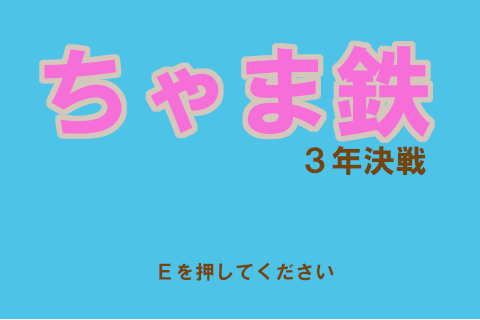
\includegraphics[scale=1.7]{sp4.png}
        \caption{タイトル画面}
         \label{title}
        \end{figure}   
    
        \begin{lstlisting}[basicstyle=\ttfamily\footnotesize, frame=single,label=startgamekey,caption=キーボードの入力制御(ゲームスタート)]
//キーボード入力管理タイマー 
void keyboardTimer(int t)
{
    // キーボード入力ロックを解除
    keyboardflg=0;
}

// eを押したか判定
// 1: キーがE
// 0 : キーがEでない
int isE(unsigned char key){
    if(key=='e'){
        return 1;
    }else{
        return 0;
    }
}

void keyboard(unsigned char key,int x,int y){
    int locktime =500;
    if(keyboardflg==0){ // キーボード入力がロックされていないとき
        if(turnstatus==0){ //タイトル
            if(isE(key)){
                inflg++;
            }
        }

        (中略)
        
        if(turnstatus!=5){
            keyboardflg=1; // キーボード入力ロック
            glutTimerFunc(locktime, keyboardTimer, 0); // ロック解除タイマー
    }
    }
}

    \end{lstlisting} 

    \subsection{目的地の設定処理}
    目的地の設定について説明する.Display関数ではturnstatusが1のときの処理である. turnstatusが1のときのキーボードの処理については
    タイトル画面と同様にEキーを押すとinflgが1インクリメントされる仕組みになっている.このため,keyboard関数のコードは省略する.
    リスト\ref{desicionDist}に目的地の設定を行う関数であるdesicionDist関数のコードを示す.
        \begin{lstlisting}[basicstyle=\ttfamily\footnotesize, frame=single,label=desicionDist,caption=desicionDist関数]
// 目的地決定処理
void desicionDist(void){
    char fname[150];
    PutSprite(spimg[2],0,0,&spinfo[2],1); // 背景表示
    if(inflg==0){
        if(goalflg==0){ // 初めて目的地をセットするとき
            // さいしょのもくてきちをきめます.
            // Eでルーレットをまわしてください.
            sprintf(fname,"saiisilonomokutekitiwokimemasumrxxxede
            llrullmsllrelttollwomawasitekudasaiimr");             
        }else if(goalflg==1){
            // つぎのもくてきちをきめます.
            // Eでルーレットをまわしてください.                
            sprintf(fname,"tuginomokutekitiwokimemasumrxxxedellru
            llmsllrelttollwomawasitekudasaiimr");                 
            }
        drawText(fname,11,225,InitWidth-22,42,0);
    }else if(inflg==1){ // 乱数生成用の設定
        dummynum=1;
        dummyresult[0]=0;
        range=STATIONNUM; // rangeを駅の数にセット
        randflg=1; // ダミータイマーロック解除
        //タイマー呼び出し
        glutTimerFunc(RANDTIME, RandTimer, 0);
        inflg++;
    }else if(inflg==2){ // ダミーリザルトを表示
        drawString(stations[dummyresult[0]].name,0,InitWidth/2-80,105,1); 
        // Eでとめます.
        sprintf(fname,"xedetomemasumr");
        drawText(fname,11,225,InitWidth-22,42,0);             
    }else if(inflg==3){
        randflg=0; // タイマー停止
        randresult=rand()%range; // 結果を計算
        // 目的地の座標,名前を格納
        distination.x=stations[randresult].x;
        distination.y=stations[randresult].y;
        sprintf(distination.name,"%s",stations[randresult].name);
        inflg++;
    }else if(inflg==4){
        // 目的地を画面出力
        // もくてきちはhogeです.
        // Eをおしてください.
        sprintf(fname,"mokutekitiha%sdesumrxxxewooositekudasaiimr",distination.name);
        drawText(fname,11,225,InitWidth-22,42,0); 
        drawString(distination.name,0,InitWidth/2-80,105,1);  
    }else if(inflg==5){ // status更新
        inflg=0;
        if(goalflg==1){
            turnstatus=7;
        }else{
            turnstatus=2;
        }
    }
}
        \end{lstlisting} 
    
        desicionDist関数の処理について説明する.
        まず,inflgの値にかかわらず行われる処理について説明する.これは背景を表示する処理のことである.
        背景を表示する処理は4行目で行っている,表示される背景は図\ref{distback}に示すものである.

        \begin{figure}[H]
            \centering
            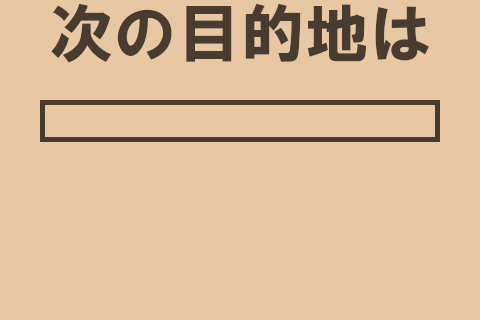
\includegraphics[scale=1.7]{sp3.png}
            \caption{目的地設定画面の背景}
             \label{distback}
            \end{figure} 
        
        inflg=0のとき,目的地を決める趣旨のダイアログを表示する処理を行っている. 表示する文字はgoalflgによって異なる.
        goalflg=0,つまり初めて目的地を決めるときは図\ref{dist1}に示すように「さいしょのもくてきちをきめます.Eでルーレット
        をまわしてください.」というダイアログが表示される. inflg=1,つまり目的地の再設定が行われるときは図\ref{dist2}に示すように
        「つぎのもくてきちをきめます.Eでルーレットをまわしてください.」というダイアログが表示される. 

        \begin{figure}[H]
            \centering
            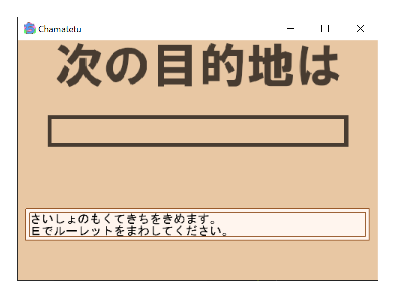
\includegraphics[scale=1.3]{distflg0.eps}
            \caption{初めて目的地を設定する場合の表示}
             \label{dist1}
            \end{figure} 
        
        \begin{figure}[H]
            \centering
            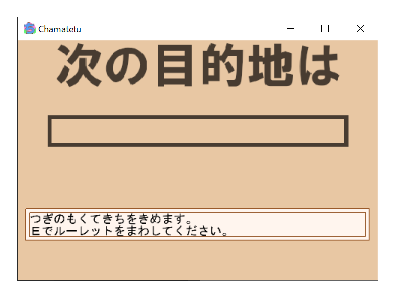
\includegraphics[scale=1.3]{distflg1.eps}
            \caption{目的地を再設定する場合の表示}
             \label{dist2}
            \end{figure} 

        ダイアログの表示方法について説明する.リスト\ref{dialog}にダイアログを表示するための関数を示す.
        リスト\ref{dialog}にはdrawDialog関数とdrawTextの2つの関数の定義が記述されている.drawDialog関数は
        ダイアログの左上の座標(x,y)から幅width,高さheightのダイアログを表示する関数である.ダイアログの描画はOpenGLのプリミティブ(図形を簡単な図形に分割して描くこと)を
        用いて行っている.描画方法は,glBegin関数とglEnd関数の間にglVertex2i関数を用いて座標を必要な数だけ並べることで
        行う.並んだ図形の結び方はglBegin関数の引数として指定する.ここでは中を塗りつぶす四角形を描画する「GL\_QUADS」と
        中を塗りつぶさない線を描画する「GL\_LINE\_LOOP」を用いている.ダイアログは3つの図形を組み合わせて表示している.
        1つ目はダイアログの背景になるペールオレンジの四角形である.これはリスト\ref{dialog}の4行目から9行目で描画している.
        2つめは外側の縁取り部分(茶色)である.これはリスト\ref{dialog}の12行目から18行目で描画している.
        3つめは内側の縁取り部分(茶色)である.これはリスト\ref{dialog}の21行目から26行目で描画している.\\
         drawText関数はダイアログの生成と文字の表示は同時に行うための関数である.リスト\ref{dialog}では29行目から
        34行目である.drawText関数は引数として受け取った文字列stringをdrawDialog関数とdrawString関数を用いて描画する
        処理を行っている. drawText関数ではダイアログと文字列が被らないようにdrawString関数の引数として与える座標(x+5,y+5)のように
        することでダイアログと表示する文字列が被らないようにする処理も行っている.
        \begin{lstlisting}[basicstyle=\ttfamily\footnotesize, frame=single,label=dialog,caption=ダイアログ表示の実装]
// ダイアログを画面に描画
void drawDialog(int x,int y,int width,int height){
    // ダイアログの背景を描画
    glBegin(GL_QUADS);
    glVertex2i(x,y);
    glVertex2i(x,y+height);
    glVertex2i(x+width,y+height);
    glVertex2i(x+width,y);
    glEnd();

    // 外側の四角を縁取り
    glColor3ub(139,69,19);
    glBegin(GL_LINE_LOOP);
    glVertex2i(x,y);
    glVertex2i(x,y+height);
    glVertex2i(x+width,y+height);
    glVertex2i(x+width,y);
    glEnd();

    // 内側の四角を縁取り
    glBegin(GL_LINE_LOOP);
    glVertex2i(x+5,y+5);
    glVertex2i(x+5,y+height-5);
    glVertex2i(x+width-5,y+height-5);
    glVertex2i(x+width-5,y+5);
    glEnd();
}

// テキスト表示
void drawText(char *string,int x,int y,int width,int height,int color){
    glColor3ub(255,245,238);
    drawDialog(x,y,width,height);
    drawString(string,color,x+5,y+5,0.5);
}
        \end{lstlisting} 

        図\ref{dist1}および図\ref{dist2}の状態でEキーを押すとinflgがインクリメントされinflg=1の処理が行われる.
        inflg=1の処理は乱数生成のための変数準備とダミーの乱数生成関数の起動である.
        inflg=1のときの処理は図\ref{desicionDist}の18行目から26行目である. 10行目ではグローバル変数dummynumに1を
        代入している.変数dummynumはdummyresult配列からいくつ結果を取り出すかを示す変数である. ダミー乱数の生成は
        複数の乱数を同時に生成したい場合があるため,dummyresult配列からいくつ結果を取り出すかで管理している.
        21行目ではグローバル変数rangeに駅の数を代入している.変数rangeは乱数の生成範囲を指定する変数である.
        変数rangeに代入した値$M$,生成される乱数$x$とすると,乱数を生成する関数では$0 \leq x < M$の範囲の
        整数乱数が生成される.22行目ではグローバル変数randflgを1にすることでダミー乱数を生成するタイマーを起動する準備をしている.
        24行目では,ダミー乱数を生成するタイマーであるRandTimer関数をコールバック関数として登録する処理を行っている.\\
         リスト\ref{RandTimer}にRandTimer関数のコードを示す. RandTimer関数の内部では, dummynum個の乱数を生成し,
        その結果をdummyresult配列に代入する処理を行っている.そして, randflgが1のときは再度RandTimer関数を呼び出す処理を行っている.
        定数RANDTIMEの値は100であるから,100msおきにRandTimer関数が呼び出される.
        \begin{lstlisting}[basicstyle=\ttfamily\footnotesize, frame=single,label=RandTimer,caption=RandTimer関数]
// ダミー乱数を一定時間ごとに生成するタイマー
void RandTimer(int t)
{ // (0,range-1)の範囲の乱数を生成
    int i;
    for(i=0;i<dummynum;i++){
        dummyresult[i] = rand()%range;
    }
    if(randflg==1){ // randflgがたっているときタイマー継続
        glutTimerFunc(RANDTIME, RandTimer, 0);
    }
}
        \end{lstlisting}
         最後にinflgをインクリメントする処理を行っている(リスト\ref{desicionDist}の25行目).
        この処理によってinflg=1の処理は一回のみ行われ,inflg=2の処理が始まる.\\
         次にinflg=2のときの処理について説明する.inflg=2のとき,生成したダミー乱数の結果を画面に出力する処理を行っている.
        図\ref{distrand1}および図\ref{distrand2}にinflg=2のときの画面表示を示す.図\ref{distrand1}および図\ref{distrand2}
        に示すように,目的地駅のダミー表示は100msおきに変化する.また,「Eでとめます.」というダイアログが表示される.

        \begin{figure}[H]
            \centering
            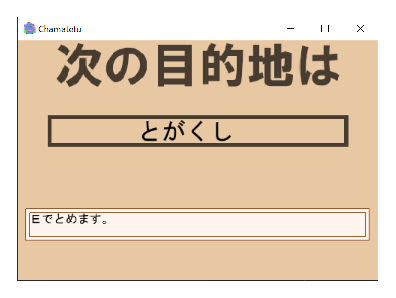
\includegraphics[scale=1.3]{distflg21.eps}
            \caption{ランダムな駅の表示例1}
             \label{distrand1}
            \end{figure} 

        \begin{figure}[H]
            \centering
            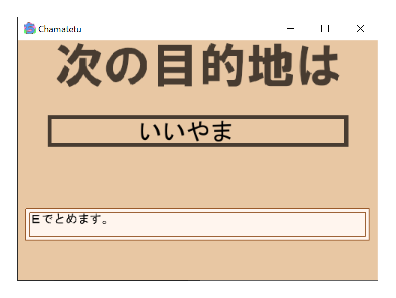
\includegraphics[scale=1.3]{distflg22.eps}
            \caption{ランダムな駅の表示例2}
             \label{distrand2}
            \end{figure} 
        
            inflg=2の処理は,リスト\ref{desicionDist}では26行目から30行目である. inflg=2のとき,
            drawString関数およびdrawText関数を用いて,ダミー乱数のインデックスに該当する駅名と
            「Eでとめます.」というダイアログを表示している.\\
             inflg=2からinflg=3への変化はキーボードのEキー入力によって行われる. inflg=3のときの処理は
            タイマーの停止とダミーでない本当の結果の計算である. リスト\ref{desicionDist}では31行目から38行目である.
            inflg=3の時の処理内容について説明する. 31行目で変数randflgを0にすることで乱数を生成するタイマーであるRandTimerが
            100msおきに呼び出される処理を停止している.これはRandTimer関数(リスト\ref{RandTimer})の8行目でrandflgが1のときに
            タイマーをコールバック関数として再登録しているためである. リスト\ref{desicionDist}の33行目では,結果として
            表示する乱数を生成しグローバル変数randresultに代入している.そして35行目から36行目で目的地の情報を保持するstationstatus
            型の変数distinationに,目的地の座標および名前を代入する処理を行っている. 最後に変数inflgをインクリメントすることでinflg=2の
            処理が1度だけ実行され,inflg=3の処理に移るようにしている.\\
             inflg=4のときの処理について説明する. inflg=4のときの処理は, inflg=3で計算して結果を画面に表示することである.これによって
            目指すべき目的地が画面に表示される.図\ref{distflg4}がinflg=4のときの画面表示の例である. 図\ref{distflg4}から読み取れるように
            inflg=4のときは,画面に目的地とダイアログが表示される. リスト\ref{desicionDist}におけるinflg=4の処理は39行目から45行目である.
            inflg=4のとき, drawText関数で「もくてきちはhogeです.Eをおしてください.」というダイアログを表示し,drawString関数で
            目的地名を表示する処理を行っている.

            \begin{figure}[H]
                \centering
                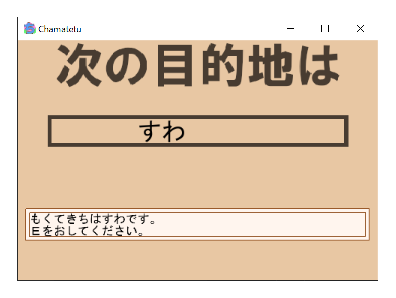
\includegraphics[scale=1.3]{distflg4.eps}
                \caption{目的地の決定}
                 \label{distflg4}
                \end{figure} 

            最後にinflg=5のときの処理について説明する. inflg=4からinflg=5への変化はEキー入力の入力によって行われる.
            リスト\ref{desicionDist}では46行目から53行目である.
            目的地を設定した後の処理は2通りある.初めての目的地設定の場合は, turnstatus=2,つまりターンのはじめの処理が
            行われる. 2回目以降の目的地の設定の場合,turnstatus=7,つまり物件の購入処理が行われる.この処理を行っているのが
            48行目から52行目である. 目的地の設定が初めてかどうかはグローバル変数goalflgが管理しているから,変数goalflgの値に
            よってturnstatusを変更する処理を行っている. これらの処理によって目的地の設定を行っている.

    \subsection{プレイヤーおよびマップの描画処理}
    プレイヤーおよびマップの描画処理について説明する. これらの処理はturnstatusが2,4,5,6,7,8,9,10で共通する処理である.
    まず,マップの描画について説明する. マップの描画はリスト\ref{drawMap}に示すdrawMap関数で行っている. マップは図\ref{map}に示したように
    960$\times$960のサイズである.これに対して,ウィンドウのサイズは480$\times$320であるため,マップ全体をウィンドウに表示することは
    できない.そこで,ターン中の社長を画面の中心に描画し,マップは社長を中心にウィンドウにおさまる範囲を描画する仕様にした.\\
        \begin{lstlisting}[basicstyle=\ttfamily\footnotesize, frame=single,label=drawMap,caption=drawMap関数]
// マップを描画
void drawMap(void){
    int x,y;
    int drawx,drawy;
    int img_num;
    for(y=0;y<InitHeight/IMGSIZE;y++){
        for(x=0;x<InitWidth/IMGSIZE;x++){
            drawx = x*IMGSIZE;
            drawy = y*IMGSIZE;
            img_num = getmapnum(x+tx,y+ty);
            if((distination.x==x+tx)&&(distination.y==y+ty)){ // 目的地のとき
                // 目的地画像を描画
                PutSprite(mapimg[DIST], drawx, drawy, &mapinfo[DIST],1);
            }else if(img_num==WALL){ // 草原マップのとき
                // 季節にあった草原を描画
                PutSprite(seasonimg[season], drawx, drawy, &seasoninfo[season],1);
            }else{
                // マップ描画
                PutSprite(mapimg[img_num], drawx, drawy, &mapinfo[img_num],1);
            }
        }
    }
}
        \end{lstlisting}

        実際の処理について説明する.まず,ターン中の社長の座標から,図\ref{mapdesc}に示すマップの左上となるMap配列のインデックス(tx,ty)を計算する.
        この値は別の関数でも仕様するため, Display関数のリスト\ref{Display}の3行目および4行目で行っている. 定数CXは7,CYは5になっている.
        このため,ターン中の社長のインデックス(x,y)から(CX,CY)を引くことで,ターン中の社長を中心としたときの
        画面左上のMap配列におけるインデックスが計算できる.drawMap関数では
        2重のfor文を用いてマップの描画を行っている. for文内の処理について説明する.リスト\ref{drawMap}の8行目および9行目では実際に
        描画する座標(drawx,drawy)を計算している.画像のサイズは32$\times$32に統一しているため,画像サイズを表す定数(IMGSIZE=32)をインデックス計算の
        ための座標(x,y)にかけることで実際の座標が計算できる.10行目では,Map配列から,描画する画像の種類を取得している. リスト\ref{getmapnum}に
        getmapnum関数の定義と, getmapnum関数内に登場する定数を示す. getmapnum関数では,引数として与えたインデックス(x,y)
        がどの種類のマスかを返す処理を行っている. 15行目から18行目では配列の添え字をはみ出したときの処理を行っている.
        配列の処理をはみ出した引数を指定した場合,背景の番号を返すように設定している.リスト\ref{drawMap}ではgetmapnum関数に
        インデックス(x+tx,y+ty)を与えることで,インデックスが(tx,ty)だけずれ,ターン中の社長を中心とするマップ描画を実現
        している.

        \begin{figure}[H]
            \centering
            
\includegraphics[scale=2.7]{mapdesc.eps}
            \caption{マップの描画方法}
             \label{mapdesc}
            \end{figure} 

        \begin{lstlisting}[basicstyle=\ttfamily\footnotesize, frame=single,label=getmapnum,caption=getmapnum関数]
// マスIDの定義
#define PLUSMASU 0 // プラス駅
#define MINUSMASU 1 // マイナス駅
#define CARDMASU 2 // カード駅
#define PROPERTYMASU 3 // 物件駅
#define SENRO1 4 // 線路(縦)
#define SENRO2 5 // 線路(横)
#define DIST 6 // 目的地駅
#define WALL 623 // 草原

// マップの画像番号を取得
int getmapnum(int x,int y){
    int img_num;
    // 配列番号をはみ出した場合
    if((x<0)||(x>=XMAX)){ 
        return 623; // 草原マップを返す
    }else if((y<0)||(y>=YMAX)){
        return 623; // 草原マップを返す
    }

    switch (Map[y][x]){
    case 'A': // 草原
        img_num=623;
        break;
    case 'B': // 物件
        img_num=3;
         break;
    case '|': // 線路(縦)
        img_num=4;
        break; 
    case '-': // 線路(横)
        img_num=5;
        break;
    case 'P': // プラス駅
        img_num=0;
        break;
    case 'M': // マイナス駅
        img_num=1;
        break;
    case 'C': // マイナス駅
        img_num=2;
        break;
    }
    return img_num;
}
        \end{lstlisting}

        表示する画像の種類を取得できたから,画像の表示を行う.リスト\ref{drawMap}では11行目から20行目の処理である.
        11行目から13行目は,例外処理として目的地駅のときに目的地駅の画像を表示する処理を行っている.14行目から16行目では
        表示する画像が背景のときの処理を行っている.背景は季節に合わせたものを表示する必要があるため,変数seasonを
        季節別の画像を格納しているseasonimg配列に渡して描画している.17行目から20行目では目的地および背景以外の
        ときの画像の描画を行っている.これらの処理によってマップを描画している.\\
         次に社長の描画方法について説明する.リスト\ref{drawPlayer}に社長を画面に表示するための関数であるdrawPlayer関数の
        コードを示す.drawPlayer関数の内部処理について説明する.drawPlayer関数はターン中ではない社長を先に描画してから,
        ターン中の社長を描画する処理を行っている. ターン中の社長を最前面に描画しないと,行動中にマップのどこにいるか分からなくなって
        しまうため,このような仕様にしている.ターン中ではない社長を描画はリスト\ref{drawPlayer}の6行目から14行目の行っている. 
        ターン中の社長かどうかは7行目のif文で判定している.ターン中の社長出ない場合は,表示する座標を計算し,PutSprite関数で描画を行っている.
        ターン中の社長の描画はリスト\ref{drawPlayer}で行っている.座標(CENTX,CNETY)は画面中心のインデックス(CX,CY)を画像サイズIMGSIZE倍した
        値である.これによって,ターン中の社長が常に画面中心に描画される.
        \begin{lstlisting}[basicstyle=\ttfamily\footnotesize, frame=single,label=drawPlayer,caption=drawPlayer関数]
// プレイヤーを描画
// 最上面にターン中のプレイヤーを描画
void drawPlayer(void){
    int transx,transy;
    int i;
    for(i=0;i<PLAYERNUM;i++){
        if(i!=turn){ // ターン中のプレイヤー以外を描画
            transx = players[i].x/IMGSIZE;
            transy = players[i].y/IMGSIZE;
            PutSprite(playerimg[i], (transx-tx)*IMGSIZE,
            (transy-ty)*IMGSIZE, &playerinfo[i],1);
        }
    }
    // ターン中のプレイヤーを最上レイヤーに表示
    PutSprite(playerimg[turn], CENTX,CENTY, &playerinfo[turn],1);
}
        \end{lstlisting}

        実際の動作について確認する.ここでは,次の3つの動作について確認する.
        \begin{enumerate}
            \item マップおよび社長が表示されるか
            \item 社長が移動したときの動作
            \item マップ端の動作
        \end{enumerate}
    
    まず,マップおよび社長が表示されるかを確認する.ここでは,ダイアログを代表とするマップと社長以外の
    表示が少ないturnstatus=5のマス移動を例に説明する.図\ref{mapplay1}にturnstatus=5のときの画面表示の例を示す.
    図\ref{mapplay1}の状況は,全社長が長野駅におり,行動中の社長はプレイヤー1社長である. レポートでは白黒のため伝わらないが,
    プレイヤー1社長が最前面に描画されている.このことから,ターン中の社長が最前面に表示される処理が正確に行えていることが確認できる.
    さらに図\ref{mapplay1}からターン中の社長が画面の中心に描画されており,マップは社長を中心に描画されていることがわかる.
    これより,社長を画面中心,マップを社長を中心に画面範囲で描画できていることが確認できる.

            \begin{figure}[H]
                \centering
                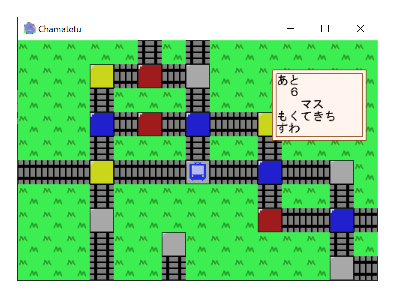
\includegraphics[scale=1.3]{mapplay1.eps}
                \caption{マップおよび社長の表示}
                 \label{mapplay1}
                \end{figure} 

    次に社長が移動したときの動作について確認する.ターン中の社長が移動すると,ターン中の社長を中心に描画したまま,
    マップの表示が変わることを確認する.図\ref{mapplay2}に社長が移動したときの画面表示を示す.図\ref{mapplay2}は
    図\ref{mapplay1}から左に128px移動した状態である.図\ref{mapplay2}から,社長が移動した場合も,
    社長が中心に表示され,マップは社長を中心に描画されることがわかる.
    \begin{figure}[H]
        \centering
        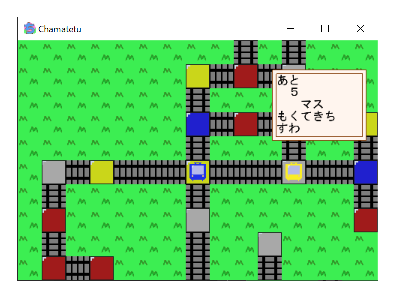
\includegraphics[scale=1.3]{maplay2.eps}
        \caption{社長が移動したときの画面表}
         \label{mapplay2}
        \end{figure} 

    最後にマップ端の動作を確認する.社長の位置によっては,マップの描画位置はMap配列の定義されている領域をはみ出す場合ある.
    この場合に背景が表示されることを確認する.図\ref{mapplay3}にプレイヤー1社長がマップ端の表示される位置に移動したときの
    画面表示を示す.図\ref{mapplay3}のプレイヤー1社長のMap配列におけるインデックスは(3,7)である.社長を中心に描画しようとすると
    画面表示の左上のMap配列におけるインデックスは(-4,2)であるため添え字をはみ出している.図\ref{mapplay3}から,添え字がはみ出している
    場合に背景が表示されていることが確認できる.これらから,ターン中の社長を中心に描画する処理と,マップをターン中の社長を中心に画面におさまる
    範囲で描画する処理について確認できた.

    \begin{figure}[H]
        \centering
        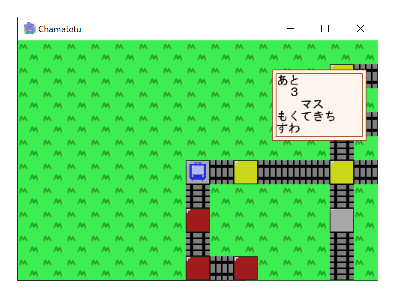
\includegraphics[scale=1.3]{maplay3.eps}
        \caption{マップ端の表示}
         \label{mapplay3}
        \end{figure} 
    
    \subsection{ターンのはじめの処理}
    ターンのはじめの処理について説明する.     
    Display関数(リスト\ref{Display})ではturnstatus=2のときの処理である.
    Display関数ではturnstatusが2のときに,startTurn関数を呼び出している.リスト\ref{startTurn}にstartTurn関数のコードを示す.
    startTurn関数の処理を,実際の動作を交えて説明する. startTurn関数の処理において,inflgの状態に関係なく実行される処理は,
    drawMap関数とdrawPlayer関数である.これらによってマップおよび社長の画像が画面に表示される. drawMap関数とdrawPlayer関数は
    次節以降でも頻繁に登場するが,使用方法は同じであるため説明は省略する.\\
     次に変数inflg=0のときの処理について説明する.リスト\ref{startTurn}では7行目から12行目である.
    変数inflg=0のときグローバル変数の初期化を行っている. グローバル変数saikoroは
    振るサイコロの数を制御するための変数である.サイコロは通常1個のみ振るが,カードの効果によって最大4個まで振ることができる仕様になっている.
    ここでは,サイコロの数を1に設定している. 11行目ではグローバル変数selectposに0を代入している.変数selectposはユーザーが選択を行う場面で
    今どれを選択しているのかを示す変数である. 変数の初期化が終了すると,12行目で変数inflgをインクリメントしてsinflg=0の状態からinflg=1
    の状態に変化させている.\\
        \begin{lstlisting}[basicstyle=\ttfamily\footnotesize, frame=single,label=startTurn,caption=startTurn関数]
// ターン開始時の処理
void startTurn(void){
    int i;
    char fname[150];
    drawMap(); // マップ描画
    drawPlayer(); // プレイヤー描画
    if(inflg==0){
        saikoro=1;
        dummynum=1;
        keyboardflg=0;
        selectpos=0;
        inflg++;
    }else if(inflg==1){
        // プレイヤーカラーでダイアログ生成
        glColor3ub(playercolor[turn][0],playercolor[turn][1],playercolor[turn][2]);
        drawDialog(11,11,InitWidth-22,34+16);
        // hogeねんめ hugaがつ
        sprintf(fname,"%dnennmess%dgatu",year,month);
        drawString(fname,0,16,11+8,0.5);
        // 所持金表示
        drawMoney(players[turn].money,InitWidth/2,11+8+16,0,0.5);
        // hogeしゃちょう
        sprintf(fname,"%ssilatilouussssss",players[turn].name);
        drawString(fname,0,16,11+8+16,0.5);   
        // サイコロ
        // カード
        sprintf(fname,"llsaiikoroxxkallmslldoll");
        drawDialog(11,175,74,42);
        // セレクトポジション表示
        if(selectpos == 0){
            glColor3ub(255,0,0);
            drawQUAD(16,180,64,16);                 
        }else if(selectpos==1){
            glColor3ub(255,0,0);
            drawQUAD(16,196,64,16);               
        }   
        drawString(fname,0,16,180,0.5);
        // hogeしゃちょうのばんです.
        sprintf(fname,"%ssilatilouunobanndesumr",players[turn].name);
        drawText(fname,11,225,InitWidth-22,42,0);      
    }else if(inflg==2){
        if(selectpos==0){
            inflg++;
        }else{
            if(players[turn].cardnum==0){
                inflg=4;
            }else{
                selectpos=0;
                inflg=5;
            }
        }
    }else if(inflg==3){ // status更新(サイコロをふる)
        inflg=0;
        turnstatus++;
    }else if(inflg==4){ // カードがないとき
        sprintf(fname,"llkallmslldollga1maiimoaarimasennmr");
        drawText(fname,11,225,InitWidth-22,42,0);               
    }else if(inflg==5){
        glColor3ub(255,245,238);
        drawDialog(155,50,10+10*16,10+16*(players[turn].cardnum+1));
        // セレクトポジション表示
        glColor3ub(255,0,0);
        drawQUAD(160,55+selectpos*16,10*16,16);                 
        
        for(i=0;i<players[turn].cardnum;i++){
            if(players[turn].card[i]!=0){
                drawString(cardname[players[turn].card[i]-1],0,160,55+i*16,0.5);                   
            }
        }
        drawString("modoru",0,160,55+players[turn].cardnum*16,0.5);
    }else if(inflg==6){
        if(selectpos==players[turn].cardnum){ // もどるのとき
            selectpos=0;
            inflg=1;
        }else{
            rcard = cardprocess(players[turn].card[selectpos]);
            inflg++;
        }
    }else if(inflg==7){
        if(rcard==0){
            // こうげきがかわされた.
            sprintf(fname,"kouugekigakawasaretamr");
            nextflg=1;
        }else if(players[turn].card[selectpos]==KYUKO){
            // サイコロが2つになった.
            sprintf(fname,"llsaiikorollga2tuninalttamr");
            nextflg=0;
        }else if(players[turn].card[selectpos]==TOKKYU){
            // サイコロが3つになった.
            sprintf(fname,"llsaiikorollga3tuninalttamr");
            nextflg=0;
        }else if(players[turn].card[selectpos]==SINKANSEN){
            // サイコロが4つになった.
            sprintf(fname,"llsaiikorollga4tuninalttamr");
            nextflg=0;
        }else if(players[turn].card[selectpos]==SAMMIT){
            // ぜんしゃちょうがhogeしゃちょうのもとにあつまった.
            sprintf(fname,"zennsilatilouuga%ssilatilouunomotoniaatumalttamr",
            players[turn].name);
            nextflg=1;
        }else if(players[turn].card[selectpos]==BUTTOBI){
            // hogeしゃちょうはいったいどこへ.
            sprintf(fname,"%ssilatilouuhaiilttaiidokohe",players[turn].name);
            nextflg=1;
        }else if(players[turn].card[selectpos]==JUOKU){
            // hogeしゃちょうにプラス10億円.
            sprintf(fname,"%ssilatilouunillpurasull10oxexmr",players[turn].name);
            nextflg=1;
        }else if(players[turn].card[selectpos]==TOKUSEIREI){
            // ぜんしゃちょうのしゃっきんがちょうけしになった.
            sprintf(fname,"zennsilatilouunosilaltkinngatilouukesininalttamr");
            nextflg=1;
        }else if(players[turn].card[selectpos]==GOUSOKKYU){
            // ほかのちゃちょうのカードがなくなった.
            sprintf(fname,"hokanosilatilouunollkallmslldollganakunalttamr");
            nextflg=1;
        }
        drawText(fname,11,225,InitWidth-22,42,0);      
    }else if(inflg==8){ // 
        // 使ったカードの消去
        for(i=selectpos;i<players[turn].cardnum-1;i++){
            players[turn].card[i]=players[turn].card[i+1];
        }
        players[turn].cardnum--;
        inflg=0;
        if(nextflg==1){
            turnstatus=15; // ターン終了 
        }else{
            turnstatus++; // サイコロをふる処理
        }     
    }
}
        \end{lstlisting}    

    inflg=1およびinflg=2のときの処理について説明する. 社長のターンが始まると図\ref{st2p1}および図\ref{st2p2}に示すような画面表示が行われる.
    図\ref{st2p1}はプレイヤー1社長の場合,図\ref{st2p2}はプレイヤー2社長の場合の画面である.図\ref{st2p1}から,ターンのはじめに
    は年月および所持金を表示するダイアログ,サイコロとカードのどちらを使用するか選択するダイアログ,「(社長名)しゃちょうのばんです.」という
    表示を行うダイアログの3つが表示されることがわかる.また,図\ref{st2p1}および図\ref{st2p2}の画面では,「W」および
    「S」キーで,サイコロとカードの選択を示す赤い四角形の位置を変化させることができる.これをセレクトポジションと
    よぶことにする.セレクトポジションはデフォルトで「サイコロ」になっており,「S」キーを押すと,図\ref{st2p3}に示す
    ように「カード」が選択された状態になる. 「カード」を選択した状態で「W」キーを押すと「サイコロ」を選択した状態になる.
    どちらかを選択した状態で「E」を押した場合の処理は後で行う.これらを実装しているのがinflg=1およびinflg=2のときの処理である.

    \begin{figure}[H]
        \centering
        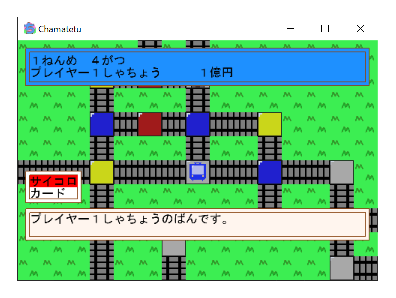
\includegraphics[scale=1.3]{st2p1.eps}
        \caption{ターンのはじめの画面(プレイヤー1社長)}
         \label{st2p1}
        \end{figure} 

        \begin{figure}[H]
            \centering
            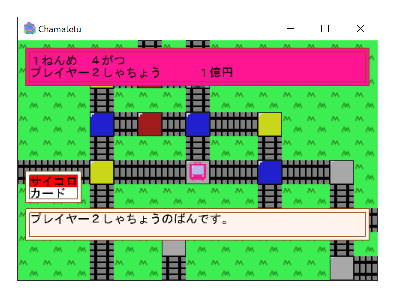
\includegraphics[scale=1.3]{st2p2.eps}
            \caption{ターンのはじめの画面(プレイヤー2社長)}
             \label{st2p2}
            \end{figure}   

        \begin{figure}[H]
            \centering
            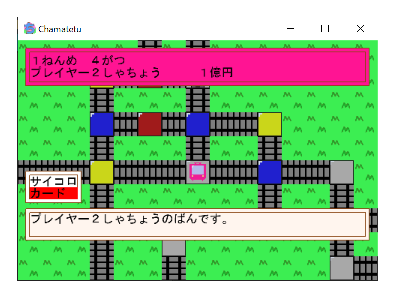
\includegraphics[scale=1.3]{st2p3.eps}
            \caption{カードを選択した状態}
             \label{st2p3}
            \end{figure}   
        
        ダイアログおよびセレクトポジションの処理を実装するコードについて説明する.リスト\ref{startTurn}では13行目から51行目である.
        inflgが1のとき,画面に先述した3つのダイアログを表示する処理を行っている.年月および所持金を表示するダイアログは15行目から
        21行目,サイコロとカードのどちらを使用するか選択するダイアログは27行目から37行目,「(社長名)しゃちょうのばんです.」という
        表示を行うダイアログは39行目および40行目である.セレクトポジションはグローバル変数selectposで管理している. 変数selectposは
        グローバル変数であるから,「W」または「S」のキーの入力があったときにkeyboard関数で変数selectposの値を変更する処理を行っている.
        リスト\ref{keyboardstatus2}にkeyboard関数におけるturnstatus=2のときの処理を示す.変数selectposの値を操作しているのは
        リスト\ref{keyboardstatus2}の9行目から20行目である. 9行目ではinflgが1かどうか判定を行っている.これは,turnstatus1のときの
        他のキーボード入力処理と区別するためである.10行目から17行目は押されたキーが「W」または「S」のキーかどうかを判定し
        変数selectposを変更する処理を行っている.変数selectposが0のとき「サイコロ」,1のとき「カード」になる仕様になっている.
        \begin{lstlisting}[basicstyle=\ttfamily\footnotesize, frame=single,label=keyboardstatus2,caption=ターンのはじめのキーボード入力の処理]
// キーボード入力管理
void keyboard(unsigned char key,int x,int y){
    int locktime =500;
    int transx = players[turn].x/IMGSIZE;
    int transy = players[turn].y/IMGSIZE;
if(keyboardflg==0){ // キーボード入力がロックされていないとき
    (省略)
    }else if(turnstatus==2){ // ターンのはじめ
    if(inflg==1){
        if(key=='w'){
            if(selectpos==1){
                selectpos=0;
            }   
        }else if(key=='s'){
            if(selectpos==0){
                selectpos=1;
            }
        }else if(isE(key)){
            inflg++;
        }
    }else if(inflg==4){
        if(isE(key)){
            inflg=1;
        }        
    }else if(inflg==5){
        if(key=='w'){
            if(selectpos>=1){
                selectpos--;
            }   
        }else if(key=='s'){
            if(selectpos<players[turn].cardnum){
                selectpos++;
            }
        }else if(isE(key)){
            inflg++;
        }        
    }else{
        if(isE(key)){
            inflg++;
        }        
    }
    }
    (省略)

    if(turnstatus!=5){
        keyboardflg=1; // キーボード入力ロック
        glutTimerFunc(locktime, keyboardTimer, 0); // ロック解除タイマー
    }
}
}
        \end{lstlisting}   

        keyboard関数でselectposの値を操作することで,リスト\ref{startTurn}の30行目のif文の真偽が変化し,どちらを選択しているか
        示すための赤い四角形を描画している.赤い四角形はdrawQUAD関数で描画している.リスト\ref{drawQUAD}にdrawQUAD関数の定義を示す.
        drawQUADは引数として,四角形を描画する左上の座標(x,y)および四角形の幅width,高さheightを受け取る.内部では,プリミティブを
        用いた描画を行うOpenGLの関数を用いて四角形の描画を行っている.

        \begin{lstlisting}[basicstyle=\ttfamily\footnotesize, frame=single,label=drawQUAD,caption=drawQUAD関数]
// 四角形を描画
void drawQUAD(int x,int y,int width,int height){
    glBegin(GL_QUADS);
    glVertex2i(x,y);
    glVertex2i(x,y+height);
    glVertex2i(x+width,y+height);
    glVertex2i(x+width,y);
    glEnd();       
}
        \end{lstlisting}   
         inflg=1の状態からinflg2の状態になる処理は, リスト\ref{keyboardstatus2}の18行目から20行目に示すようにEキーの
        入力によるinflgのインクリメントによって行っている.inflgが2のときの処理(リスト\ref{startTurn}の41行目から51行目)は,
        Eキーを押したときのセレクトポジションによって処理を分岐する処理である. セレクトポジションが「サイコロ」,つまり変数selectpos=0
        の場合はinflgを3にしている. セレクトポジションが「カード」,つまり変数selectposが1の場合はカード枚数を確認し,
        カード枚数が0のときinflgを4,そうでないときはinflgを5にしている.\\
         inflg=3のときの処理について説明する.リスト\ref{startTurn}では52行目から54行目である.
        inflgが3のときの処理はサイコロを振る処理にturnstatusの値を変更することである.turnstatus=3は未使用であるが,
        ここではturnstatusをインクリメントする処理を行っている.\\
         inflg=4のときの処理を説明する.inflg=4の処理はカードが1枚もないときに,「カード」が選択された時の処理である.
        この場合,図\ref{nocard}に示すように「カードが1まいもありません.」と画面に表示される.リスト\ref{startTurn}では55行目から57行目である. 
        図\ref{nocard}の状態で,Eキーを押すとリスト\ref{keyboardstatus2}の21行目から24行目に示す処理によってinflg=1,つまり図\ref{st2p1}
        に示す画面に戻る.

     \begin{figure}[H]
        \centering
        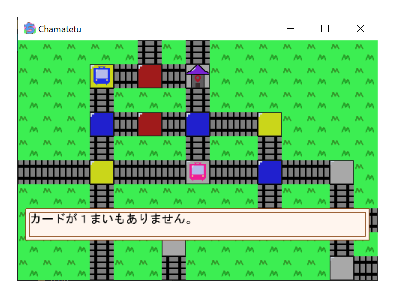
\includegraphics[scale=1.3]{st2fl4.eps}
        \caption{カードが1枚もないときのカード表示}
         \label{nocard}
        \end{figure}        

        最後に,inflgが5~8のときの処理について説明する. inflgが5~8のときの処理は図\ref{st2p1}で「カード」を選択したときの処理である.
        カードを持っている場合に「カード」を選択すると図\ref{havecard}に示すように,手持ちのカードが表示される.図\ref{havecard}の例では
        「サミットカード」,「とっきゅうカード」,「ごうそっきゅうカード」の3種類を持っている.また,一番下のセレクトポジションには「もどる」
        という項目がある.いずれかのカードを選択した状態でEキーを押すと,カードが使用される.「もどる」を選択してEキーを押すと
        図\ref{st2p1}の画面に戻る.

        \begin{figure}[H]
            \centering
            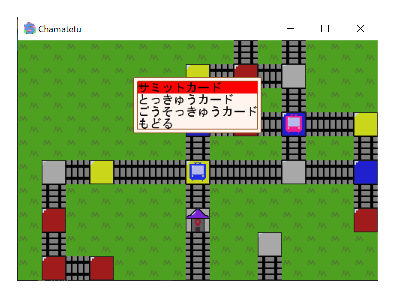
\includegraphics[scale=1.3]{havacard.eps}
            \caption{手持ちのカードの表示}
             \label{havecard}
            \end{figure}   
        
        これらがinflgが5~8のときの処理である.リスト\ref{startTurn}では58行目から122行目である.
        「カード」が選択されるとまずinflg=5の処理が行われる. リスト\ref{startTurn}では58行目から70行目である. 
        inflg=5の処理は,手持ちのカード,「もどる」,セレクトポジション
        の3つ画面に表示する処理である.手持ちのカードはplayerstatus型の配列playersのメンバcardが保持しているから,drawString関数で
        これを表示している. inflg=5でのセレクトポジションの処理はリスト\ref{keyboardstatus2}の25行目から41行目に記述されている.
        セレクトポジションの移動処理は「カード」,「サイコロ」を選択するときの処理と同じであるため,説明は省略する.\\
         カードを選択してEキーを押すとinflg=6の処理が行われる. リスト\ref{startTurn}では71行目から78行目である. 
        ターン中の社長のカード枚数$c$とすると,変数selectposの値sが$0 \leq s \leq c-1$ のときは,所持しているカードのいずれかが
        選択されているため,カードの効果を発動する関数であるcardprocess関数を実行している.変数selectposの値がターン中の社長のカード枚数と
        等しいとき,「もどる」が選択されているためinflg=1,つまり図\ref{st2p1}の画面に戻るようにしている.\\
         カードの効果を発動する関数である
        cardprocess関数について説明する.リスト\ref{cardprocess}にcardprocess関数のコードを示す.cardprocess関数は引数として
        効果を発動するカードの番号を受け取る.また,返り値としてカードの発動が成功した場合に1,失敗した場合に0を返す.カードの番号と発動するカードはリスト\ref{cardprocess}の2行目から10行目のようになっている.
        各カードの処理について説明する.発動するカードが,急行カード,特急カード,新幹線カードのいずれかのときサイコロの数を管理するグローバル変数saikoro
        の値を更新する処理を行っている.サイコロの数は急行カードのときは2個,特急カードのときは3個,新幹線カードのときは4個にしている.\\
         サミットカードの場合は,成功または失敗の計算をしたのちに,カードの効果を発動している.確率$\frac{2}{3}$で成功するために,乱数を生成して
        3で割った値が0でないときにカードの効果を発動するようにしている.サミットカードの効果は,すべての社長をターン中の社長の駅に集める効果
        であるから,全ての社長の座標をターン中の社長の座標で上書きする処理を行っている.ぶっとびカードの効果は社長をランダムな物件駅に飛ばす効果であるから,物件駅の数を表す定数STATIONNUMで乱数をわることで,
        ランダムな駅のインデックスを取得している.そして,取得したインデックスに該当する物件駅の座標をstations構造体から取得して
        画像サイズIMGISIZE倍することで,新しい座標が計算される.この座標をターン中の社長の座標に代入することで,ランダムな駅へぶっとぶ
        効果を実装している. 10億円カードは使用すると10億円が手に入るカードであった.10億円カードの時の処理は,ターン中の社長の
        moneyをプラス100000する処理ことで10億円を所持金に追加している.徳政令カードは借金を負っている社長の所持金を0にするカードであった.このため,全ての社長について所持金を保持するメンバmoneyが
        0よりも小さいか判定し,0よりも小さい場合はメンバmoneyを0にする処理を行っている.剛速球カードは確率$\frac{1}{2}$で成功し,他の社長のカードを全て破棄するカードであった.このため,生成した乱数を2で割り0のとき
        はターン中の社長以外のカード配列およびカード枚数を0で埋める処理を行っている.これらの処理によってカードの効果を実装している.
        \begin{lstlisting}[basicstyle=\ttfamily\footnotesize, frame=single,label=cardprocess,caption=cardprocess関数]
// カード番号の定義
#define KYUKO 1 // 急行カード
#define TOKKYU 2 // 特急カード
#define SINKANSEN 3 // 新幹線カード
#define SAMMIT 4 // サミットカード 
#define BUTTOBI 5 // ぶっとびカード
#define JUOKU 6 // 十億円カード
#define TOKUSEIREI 7 // 徳政令カード
#define GOUSOKKYU 8 // 剛速球カード

// カード処理
int cardprocess(int num){
    int r=1;
    int i,j,randst;
    if(num==KYUKO){ // 急行カード
        saikoro=2;
    }else if(num==TOKKYU){ // 特急カード
        saikoro=3;
    }else if(num==SINKANSEN){ // 新幹線カード
        saikoro=4;
    }else if(num==SAMMIT){ // サミットカード
        if(rand()%3!=0){
            for(i=0;i<PLAYERNUM;i++){
                players[i].x=players[turn].x;
                players[i].y=players[turn].y;
            }
        }else{
            r=0;
        }
    }else if(num==BUTTOBI){ // ぶっとびカード
        randst = rand()%STATIONNUM;
        players[turn].x = stations[randst].x*IMGSIZE;
        players[turn].y = stations[randst].y*IMGSIZE;
    }else if(num==JUOKU){ // 10億円カード
        players[turn].money+=100000;
    }else if(num==TOKUSEIREI){ // 徳政令カード
        for(i=0;i<PLAYERNUM;i++){
            if(players[i].money<0){
                players[i].money=0;
            }
        }
    }else if(num==GOUSOKKYU){ // 剛速球カード
        if(rand()%2){
        for(i=0;i<PLAYERNUM;i++){
            if(i!=turn){
                players[i].cardnum=0;
                for(j=0;j<CARDMAX;j++){
                    players[i].card[j]=0;
                }
            }
        }
        }else{
           r=0; 
        }        
    }
    dummynum=saikoro;
    return r;
}
        \end{lstlisting}   
         カードの発動の成功/失敗はリスト\ref{startTurn}の76行目に示すように変数rcardに保存される.
        カードの処理が終了すると,リスト\ref{startTurn}の77行目に示すように,inflgがインクリメントされinflg=7の処理が行われる.
        inflg=7のときの処理について説明する. inflg=7の処理はカードを使用した結果を画面に表示する処理である. 
        図\ref{c1}~図\ref{c9}に各カードを使用したときの画面表示を示す.図\ref{c1}~図\ref{c8}はカードの使用に成功した場合,
        図\ref{c9}はカードの使用に失敗した場合である.使用したカードによって表示する内容が変化する処理はリスト\ref{startTurn}の
        80行目から117行目に記述されている.また,グローバル変数nextflgの値を急行カード,特急カード,新幹線カードのいずれかのカードのとき0,
        それ以外のカードのとき1になるようにする処理を行っている.急行カード,特急カード,新幹線カードの3つのカードはカードを使用した
        後にサイコロを振るため,変数nextflgを使用して,使用したカードの判別を行っている.

        \begin{figure}[H]
            \centering
            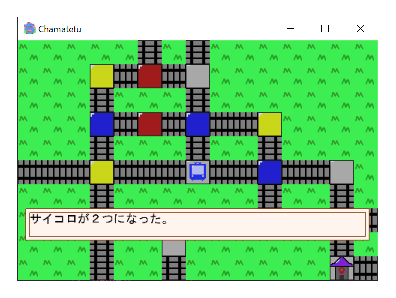
\includegraphics[scale=1.3]{kyukou.eps}
            \caption{急行カードを使用したときの表示}
             \label{c1}
            \end{figure}   

        \begin{figure}[H]
            \centering
            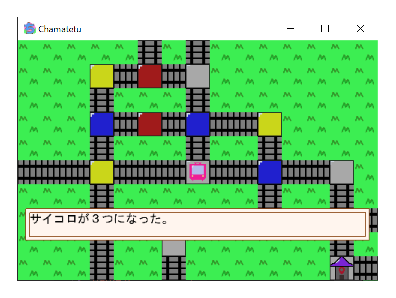
\includegraphics[scale=1.3]{tokkyu.eps}
            \caption{特急カードを使用したときの表示}
             \label{c2}
            \end{figure}  

            \begin{figure}[H]
                \centering
                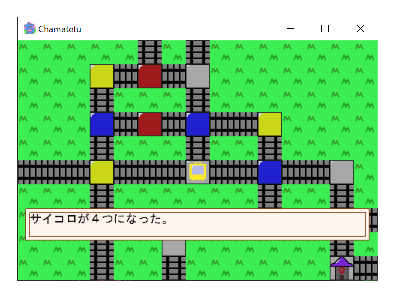
\includegraphics[scale=1.3]{sinkansen.eps}
                \caption{新幹線カードを使用したときの表示}
                 \label{c3}
                \end{figure}

        \begin{figure}[H]
            \centering
            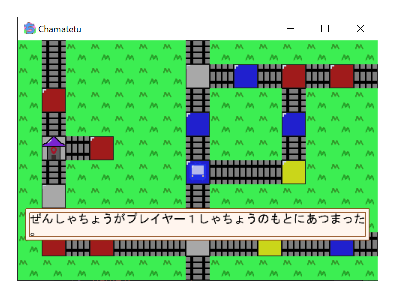
\includegraphics[scale=1.3]{samitto.eps}
            \caption{サミットカードを使用したときの表示}
             \label{c4}
            \end{figure}
            
        \begin{figure}[H]
            \centering
            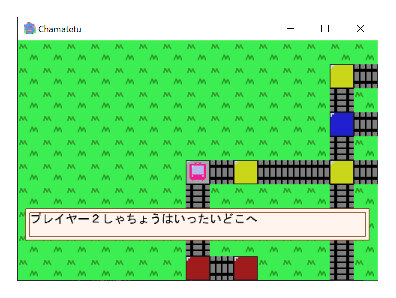
\includegraphics[scale=1.3]{buttobi.eps}
            \caption{ぶっとびカードを使用したときの表示}
             \label{c5}
            \end{figure}

        \begin{figure}[H]
            \centering
            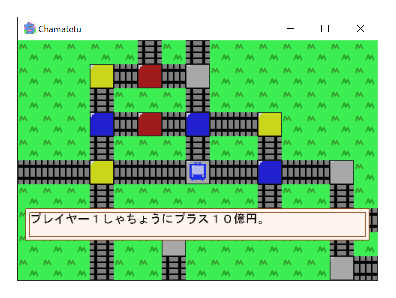
\includegraphics[scale=1.3]{tenoku.eps}
            \caption{10億円カードを使用したときの表示}
             \label{c6}
            \end{figure}

        \begin{figure}[H]
            \centering
            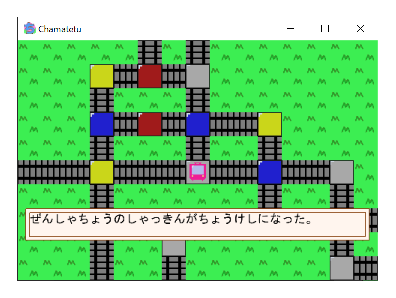
\includegraphics[scale=1.3]{tokuseirei.eps}
            \caption{徳政令カードを使用したときの表示}
             \label{c7}
            \end{figure}

            \begin{figure}[H]
                \centering
                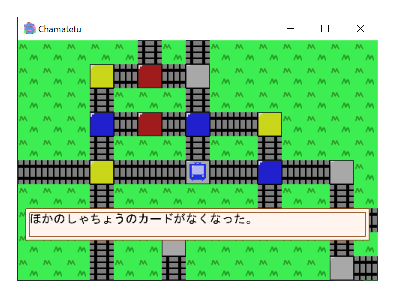
\includegraphics[scale=1.3]{kyu.eps}
                \caption{剛速球カードを使用したときの表示}
                 \label{c8}
                \end{figure}

                \begin{figure}[H]
                \centering
                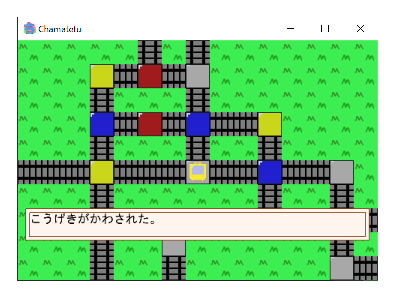
\includegraphics[scale=1.3]{hirari.eps}
                \caption{カード使用が失敗したときの表示}
                 \label{c9}
                \end{figure}

    使用したカードの種類別の画面出力が行われた状態でEキーを押すとinflg=7の状態からinflg=8の状態に変化する.
    inflg=8の処理は,使用したカードの消去とturnstatusの変化の処理である.リスト\ref{startTurn}では119行目から131行目である.
    カードの消去は121行目から124行目で行っている. turnstatusの変化の処理は126行目から130行目で行っている.
    nextflgが1のとき,サイコロを増やすカードが仕様されたことを示しているためturnstatusを4,つまりサイコロを振る処理にセットしている.
    nextflgが0のときはturnstatusを15,つまりターン終了処理にセットしている.これらの処理によってターンのはじめの処理を実装している.

    \subsection{サイコロをふる処理}
    \subsection{マス移動および停車駅の判定処理}
    \subsection{物件駅の処理}
    \subsection{プラス駅の処理}
    \subsection{マイナス駅および借金の処理}
    \subsection{カード駅の処理}
    \subsection{ターン終了時の処理}
    \subsection{決算および最終成績の処理}
    
    \section{付録 ソースコード}

    \begin{thebibliography}{9}
        \bibitem{mmtt}  桃太郎電鉄,\url{https://www.konami.com/games/momotetsu/teiban/} ,閲覧日2021年1月5日
        \end{thebibliography}
\end{document}

